%%%%%%%%%%%%%%%%%%%%%%%%%% 
\subsection{Introduction}
\label{sec:selec_motiv}
The core of this PhD project is the developpment of the analysis of MBTA's single detector triggers, not just as part of concidences, but as standalone candidate events.
The goal is to make the background low enough so we can retrieve as many astrophysical candidates as possible and compute the FAR of the candidates.

It is difficult to predict what the background will be like during O4.
We can base our investigation on the O3 background as it is the best we have and the sources of noise will not be fundamentally different.
Figure \ref{fig:compare_bkg} shows the ranking statistics background distribution for single detector triggers during double or triple detector time and the background for HL coincidences.
By comparing them we can see that high ranking statistics values are present in the single detector triggers distributions and not in the coincidence distribution.
These triggers are therefore due to noise.
We need to get rid of them if we want to claim and release significant detections for single detector triggers.
%
\begin{figure}[ht]
  \centering
  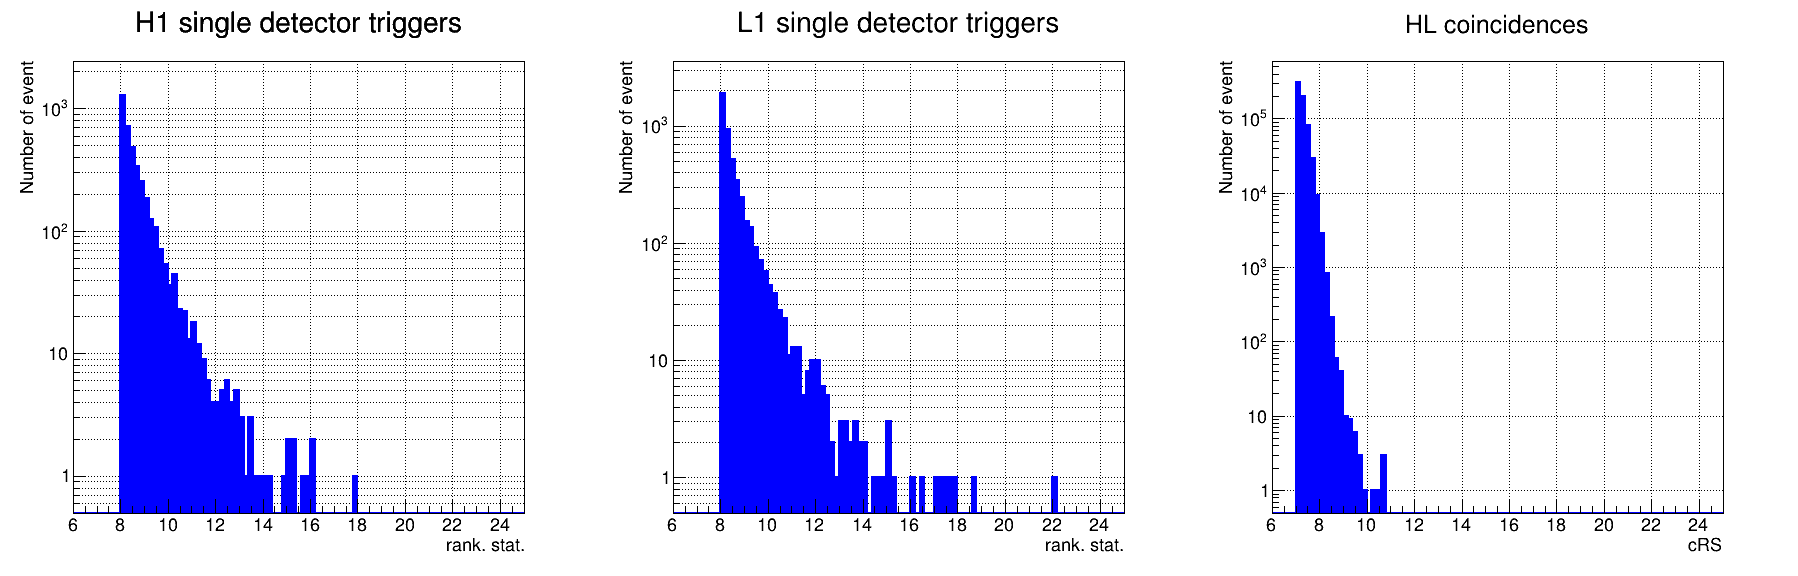
\includegraphics[width=\linewidth]{sectionSelection/plotsOther/cCompareSingleCoinc.png}
  \caption{Left and middle: single detector triggers ranking statistics distribution in H and L during O3 double and triple detector time. Right: combined ranking statistics distribution of HL triggers during the same times.}
  \label{fig:compare_bkg}
\end{figure}
%

We ask the following question: Can we use selection criteria based on pipeline-related quantities to discriminate against triggers of ``poor'' quality and effectively reduce the background?
Considered quantities were the \achi (eq. \ref{eq:achi2}), the excess rate (eq. \ref{eq:ER}) and the gating (section \ref{sec:gating}).
The criteria defined in this section do not impact the filtering of the data and can be applied as a post-processing step.
%Cutting on the \achi proved to be useless and will therefore not be discussed any further.

Since reducing the background is difficult we may also wonder whether all kind of triggers are equally interesting.
Multi-messenger considerations have a lot of weight, especially from the point of view of online analyses.
Although the sky localization of a single detector trigger is bound to be poor, especially during single detector time, the timing information still has a high scientific value in case another observatory detects some signal at the same time.
BNS and NSBH events are also rarer than BBH events so every additional detection has a lot of value.
This advocates for an emphasis on EM bright candidates that will be presented in section \ref{sec:embright}.
Another consideration in favor of EM bright candidates is that they are associated to longer signals due to their lower mass (see section \ref{sec:selec_param_space}), and are therefore easier to identify.
But it does not mean that EM-dark triggers should be excluded by default.
We will also study them in parallel to the EM bright population, to prepare a possible extension of the single detector triggers analysis to all type of sources.

This chapter starts by giving some details on the Gaussian noise mentioned previously.
This Gaussian noise will be used throughout the chapter.
We then define the EM-bright population for the MBTA single detector triggers search.
We will also develop some considerations on the importance of the duration of the templates.
This will be followed by a study on a selection using the \achi and excess rate.
There will then be further considerations which lead to consider the gating and to be more strict on the presence of excess rate around triggers to exclude times when one interferometer misbehaves.

%%
% It is difficult to predict what the background will be like during O4 but the one from O3 exhibits large tails in the SNR distribution (figure \ref{fig:O3_singles_1}) which require cleaning if we want to have confident releases for single detector triggers.
% In this section we will describe selection criteria which could be used during O4 for a single detector triggers search.
% This study is based on the full O3 offline analysis used for the GWTC-2.1 \cite{gwtc2.1} and GWTC-3 \cite{gwtc3} catalogues.
% It uses also a dedicated processing of four chunks of simulated data roughly equivalent to the duration of O3 chunks 1 to 4.
% The simulated data is Gaussian noise, which represent an ideal case of noise, generated with the typical O3 sensitivity.
% The results of the analyses of those chunks of Gaussian noise were scaled to the total observation time of O3.

% The initial observation which motivated this work is the following: for a chunk of Gaussian noise, the SNR distribution barely reaches values of 8 while we observe tails in real data distributions that go way further (figures \ref{fig:gaussian_noise} and \ref{fig:O3_singles}).
% This can be explained by the presence of loud transients (glitches) as mentionned previously in this document, as well as PSD fluctuations as discussed earlier in \ref{sec:triggers_PSD}.
% The question we ask here is the following: can we use cuts on pipeline-related quantities to discriminate against triggers of "poor" quality and effectively reduce the background?
% Considered quantities were the \achi (\ref{eq:achi2}), the excess rate (\ref{eq:ER}), the gating and the duration of the template associated to the trigger.
% Cutting on the \achi proved to be useless and will therefore not be discussed any further.
% We will start by having a look at the parameter space we want to focus on for the single detector triggers analysis and why, we will then follow with a study on a selection using the excess rate and then further consideration which lead us to be more strict on the presence of excess rate around triggers and also consider the gating.
% The template duration will not be used as a selection criteria per se but rather as a way to fragment our parameter space.



%%%%%%%%%% 
\subsection{Ideal case of noise}
\label{sec:gaussian_noise}
We want, through the application of selection criteria, to reduce the background as much as possible.
A reference for ``good'' or ``clean'' background is the ideal case where the detector strain is stationary Gaussian noise.
Background obtained by running MBTA on such noise is the limit of what we can hope to achieve.

To simulate the strain observed by a  perfect GW detector, we start by simulating stationary white Gaussian noise, i.e. time-independent noise with mean 0, standard deviation 1 and constant PSD.
It is then colored using the detectors O3b PSD.
An example of stationary gaussian noise colored with L1 PSD is shown in figure \ref{fig:colored_gaus}.
The Gaussian noise used throughout this section is computed for an effective time equivalent to the effective observing time of the first month of O3.

This Gaussian noise was analyzed with MBTA using the pipeline's O3b configuration.
In order to compare the background obtained by MBTA on this Gaussian noise to the background observed during O3, the number of triggers was scaled using the effective time ratio $T_{eff}$(O3)/$T_{eff}$ (Gaussian noise).
Histograms of the single detector triggers produced by analyzing this simulated Gaussian noise with MBTA are shown in figure \ref{fig:gaussian_noise}.
Unlike in figure \ref{fig:compare_bkg}, the Gaussian noise barely reaches rwSNR values of 8 while the O3 background has much higher values.
This confirms that an excess of significant noise triggers is present in MBTA's single detector triggers.
This Gaussian noise analysis will be a reference for the effectiveness of the selection criteria defined in this chapter.

\begin{figure}[hb]
  \centering
  \begin{minipage}{0.45\linewidth}
    \centering
    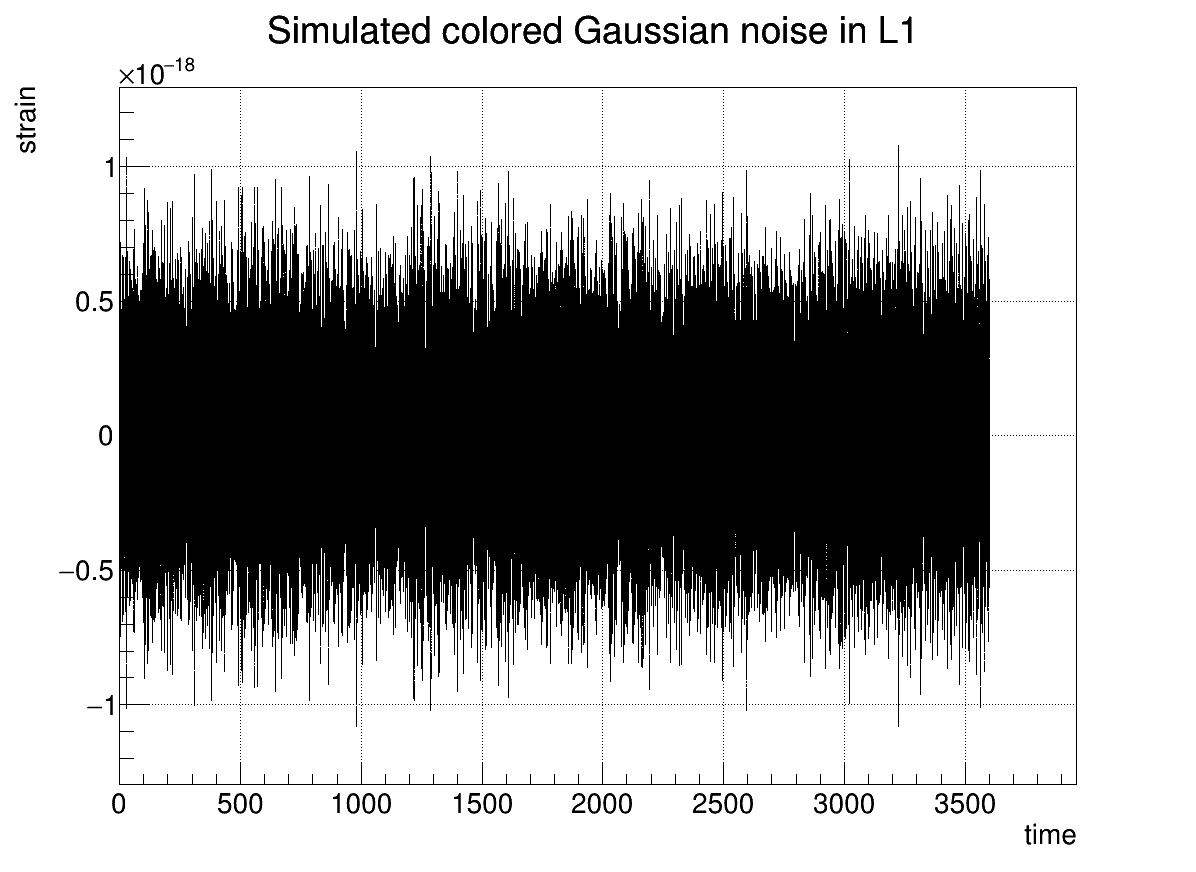
\includegraphics[width=\linewidth]{sectionSelection/plotsOther/cNoise.png}
  \end{minipage}
  \hfill
  %
  \begin{minipage}{0.45\linewidth}
    \centering
    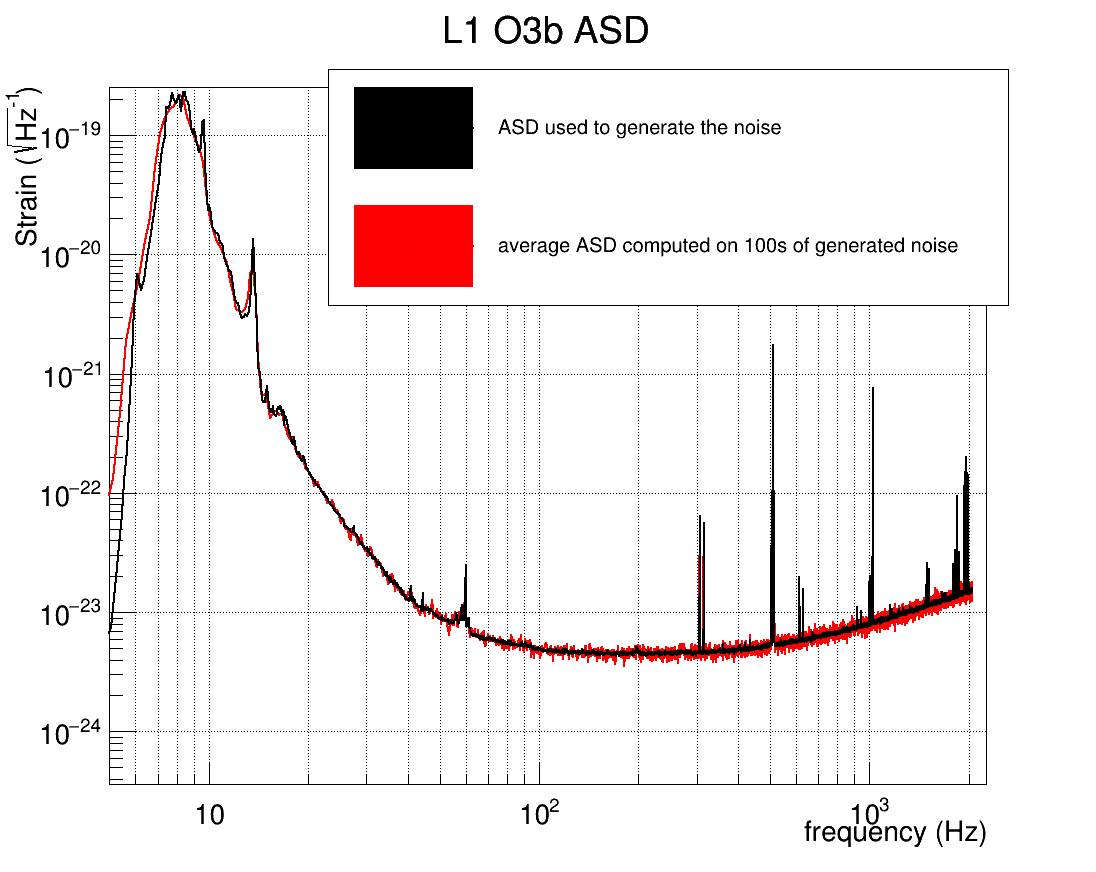
\includegraphics[width=\linewidth]{sectionSelection/plotsOther/cASDL1.png}
  \end{minipage}
  \caption{Left: One hour of simulated stationary colored Gaussian noise. Right: L1 O3b Amplitude Spectral Density ($\text{ASD}=\sqrt{\text{PSD}}$) used to color the noise and average ASD computed on 100s of the simulated noise.}
  \label{fig:colored_gaus}
\end{figure}

%
% Gaussian noise distribution
\begin{figure}[hb]
  \centering
  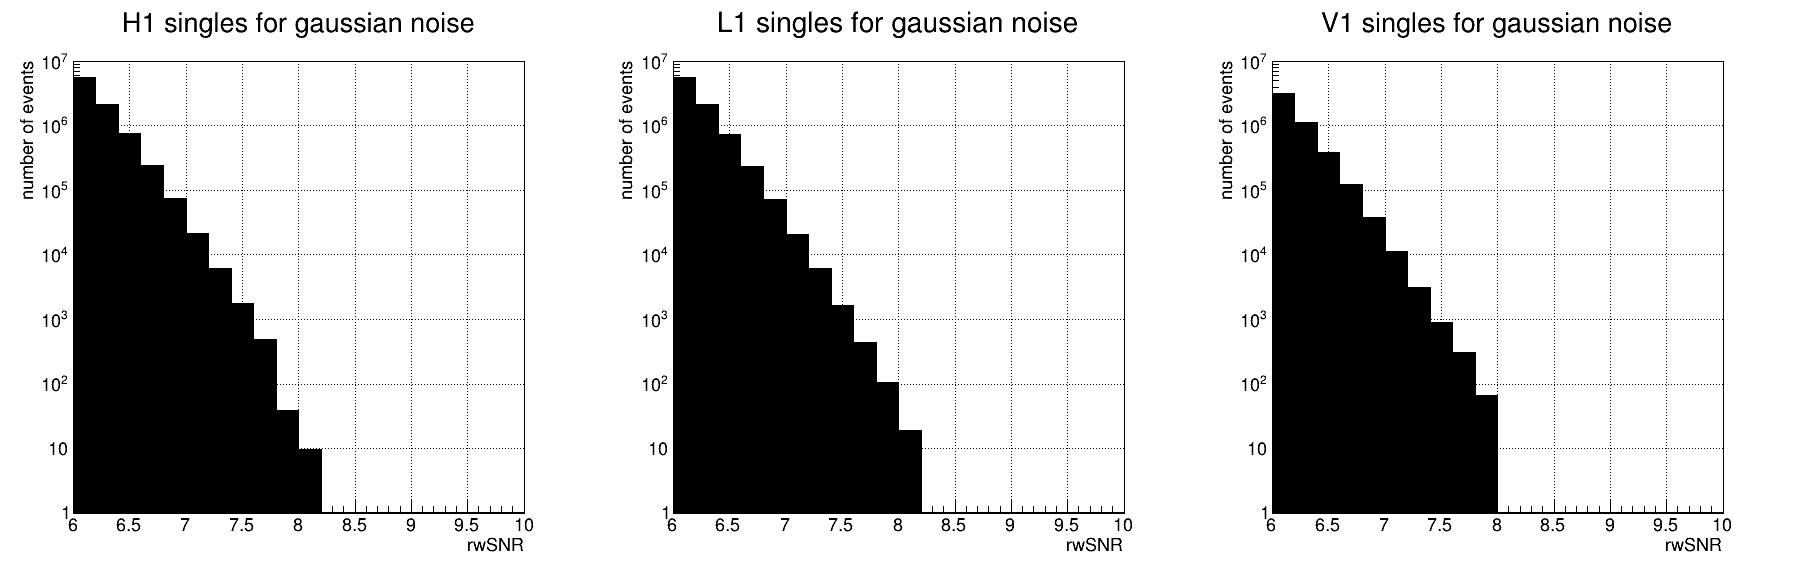
\includegraphics[width=\textwidth]{sectionSelection/plotsOther/cGausSingles.png}
  \caption{Single detector triggers for the BNS search region of a simulated Gaussian noise computed on about a month of simulated strain, scaled to the O3 effective observing time. Scaling factor for H1, L1 and V1 are 9.36, 9.13 and 9.06 respectively.}
  \label{fig:gaussian_noise}
\end{figure}




%%%%%%%%%%
\clearpage\newpage
\subsection{Monte Carlo simulations of astrophysical signals}
\label{sec:inj}

To test the efficiency of the pipeline or of some tools on a large number of astrophysical events, we rely on Monte Carlo simulations.
The simulated waveforms cover a large parameter space.
These signals are then added to the real data of the detector and are called injections.

We can then analyze those data with injections using MBTA to see which injections were found and missed.
An injection is considered as found, or recovered, if it passes the SNR (or cRS) threshold of the search and it is found within $\pm \SI{100}{ms}$ of the injected time.
Note that the PSD used for the filtering and the FAR vs cRS distributions are computed on the data without injections.

During the online analysis of O3, MBTA generated its own injections to validate the proper behaviour of the pipeline.
%MBTA generated its own injections for O3.
%They were used during the offline analysis.
%Figure \ref{fig:injections_recovery} shows the recovery of BNS injections as a function of the injected chirp mass, combined SNR and distance from GPS$=1258755060$ to GPS$=1259423400$.\textcolor{red}{vraiment utile ?}

% The parameters of MBTA injections used during O3 are given in table \ref{tab:inj}.
% %
% \begin{table}[hb]
%   \centering
%   \begin{tabular}{c|c|c|c|c}
%     type & masses & spins & distance & frequency\\ \hline
%     BNS  & \begin{tabular}{c} $m_1$ $\in$ [1,2]\msun\\ $m_2$ $\in$ [1,2]\msun \\ $m_{\text{tot}}$ $\in$ [2,4]\msun\end{tabular}
%          & \begin{tabular}{c} s$_1$ $\in$ [0,0.05]\\ $s_2$ $\in$ [0,0.05] \end{tabular}
%          & [10,300]Mpc & [24,4096]Hz\\ \hline
    
%     NSBH & \begin{tabular}{c} $m_1$ $\in$ [2,99]\msun\\ $m_2$ $\in$ [1,2]\msun \\ $m_{\text{tot}}$ $\in$ [3,100]\msun\end{tabular}
%          & \begin{tabular}{c} s$_1$ $\in$ [0,0.997]\\ $s_2$ $\in$ [0,0.05] \end{tabular}
%          & [10,600]Mpc & [22,4096]Hz\\ \hline
    
%     BBH (light)  & \begin{tabular}{c} $m_1$ $\in$ [2,99]\msun\\ $m_2$ $\in$ [2,99]\msun \\ $m_{\text{tot}}$ $\in$ [4,100]\msun\end{tabular}
%          & \begin{tabular}{c} s$_1$ $\in$ [0,0.997]\\ $s_2$ $\in$ [0,0.997] \end{tabular}
%          & [10,4000]Mpc & [20,4096]Hz\\ \hline
    
%     BBH (heavy)  & \begin{tabular}{c} $m_1$ $\in$ [2,195]\msun\\ $m_2$ $\in$ [2,195]\msun \\ $m_{\text{tot}}$ $\in$ [100,195]\msun\end{tabular}
%          & \begin{tabular}{c} s$_1$ $\in$ [0,0.997]\\ $s_2$ $\in$ [0,0.997] \end{tabular}
%          & [10,4000]Mpc & [20,4096]Hz\\ \hline
%   \end{tabular}
%   \caption{Parameters of MBTA's O3 injections. BNS injections were generated using the SpinTaylorT4threePointFivePN waveform, NSBH and BBH were generated using SEOBNRv4pseudoFourPN.}
%   \label{tab:inj}
% \end{table}
%

To compare pipelines' performances with each other, a set of common injections was made by the rates and populations LVK group.
They were added on top of the full O3 data and processed by MBTA with the regular search configuration.

The BBH common injections were generated as follow:
\begin{itemize}
\item $2<m_{1,2}< \SI{100}{\msun}$, proba$(m_1) \propto m_1^{-2.35}$, proba$(m_2) \propto m_2$
\item $|s_{1,2}|<0.998$, uniform in spin magnitude, isotropic in spin orientation
\item redshift $z<1.9$, proba$(z) = d($comoving volume$)/dz \times d(t_{\text{source}})/dt \times (1+z)$
\item frequency$\in [10,1500]$ Hz
\end{itemize}
\vspace{0.2cm}
%
For the BNS common injections:
\begin{itemize}
\item $1<m_{1,2}<\SI{2.5}{\msun}$, uniformly distributed
\item $|s_{1,2}|<0.4$, uniform in spin magnitude, isotropic in spin orientation
\item redshift $z<0.15$, uniform in comoving volume-time
\item frequency$\in [15,1500]$ Hz
\end{itemize}
\vspace{0.2cm}
%
Finally for the NSBH common injections:
\begin{itemize}
\item $2.5<m_{1}<\SI{60}{\msun}$, following a Salpeter power law with slope $-2.35$
\item $1<m_{2}<\SI{2.5}{\msun}$, uniformly distributed
\item $|s_{1}|<0.998$, $|s_{2}|<0.4$, uniform in spin magnitude and isotropic in spin orientation for both
\item redshift $z<0.25$, uniform in comoving volume-time
\item frequency$\in [15,1500]$ Hz
\end{itemize}

BNS injections were generated using the SpinTaylorT4threePointFivePN waveform, NSBH and BBH were generated using SEOBNRv4pseudoFourPN.
Figure \ref{fig:common_inj} shows the masses and distance distribution of the O3 common injections.

% \begin{figure}
%   \centering

%   \begin{minipage}{\linewidth}

%     \begin{minipage}{0.45\linewidth}
%       \centering
%       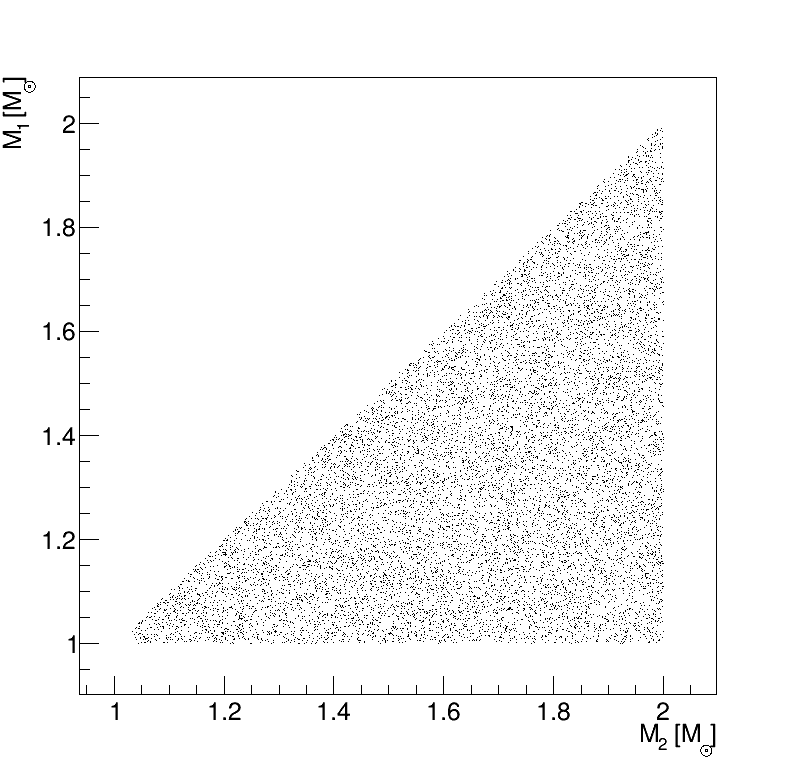
\includegraphics[width=\linewidth]{sectionSelection/plotsOther/inj_masses_chunk26.png}
%     \end{minipage}
%     \hfill
% \begin{figure}
%   \centering
%   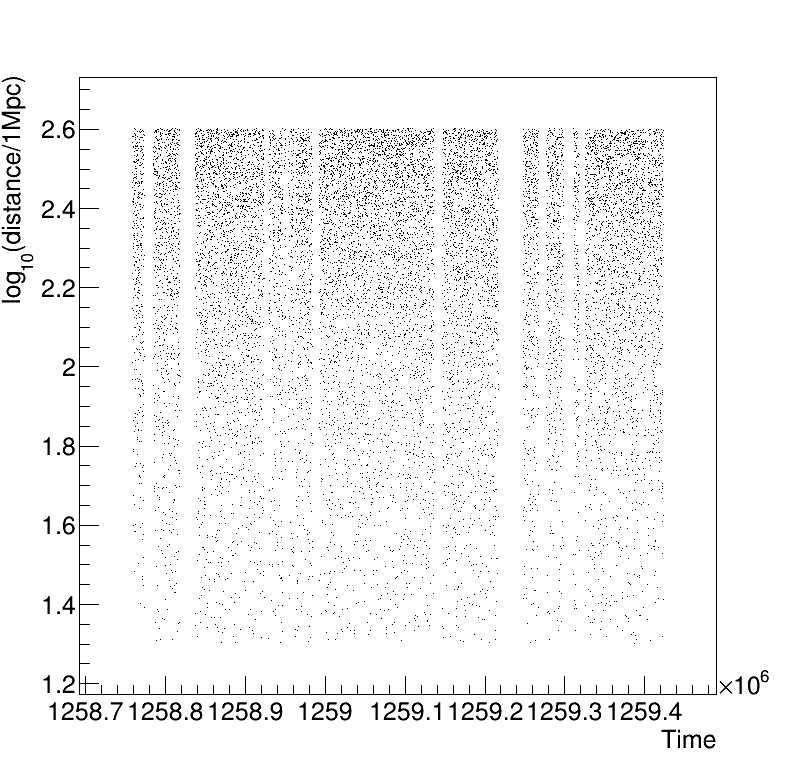
\includegraphics[width=\linewidth]{sectionSelection/plotsOther/inj_time_chunk26.png}
%   \hfill
%   \caption{Plots of the MBTA production monitoring for BNS injections on around 6 days. Missed and found injections in SNR and distance.}
%   \label{fig:injections}
% \end{figure}
% % \end{figure}

% \begin{figure}
%   \centering
%   \begin{minipage}{\linewidth}
%     \centering
%     \begin{minipage}{0.45\linewidth}
%       \centering
%       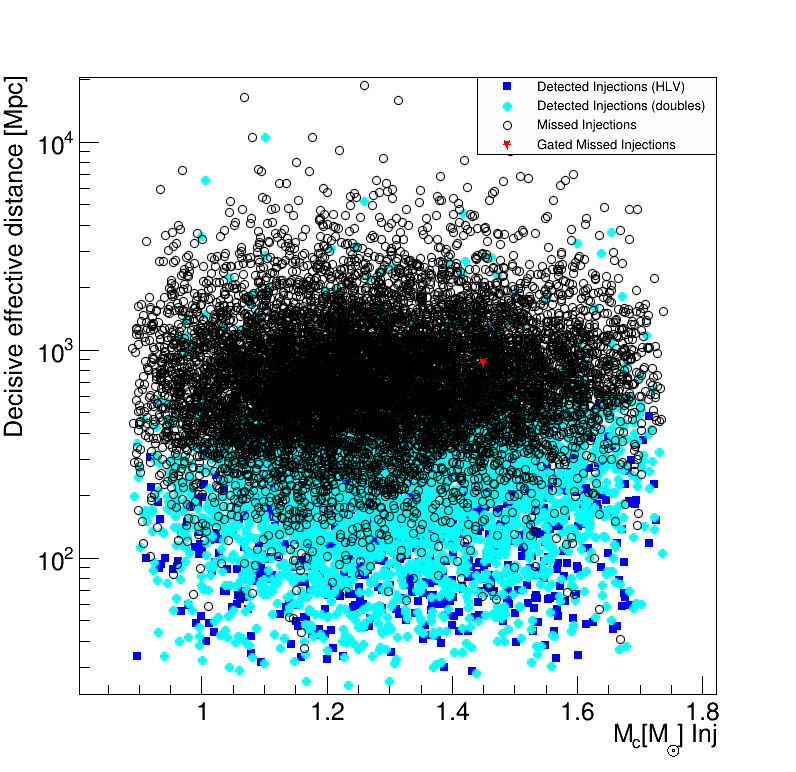
\includegraphics[width=\linewidth]{sectionSelection/plotsOther/inj_recovery_mc_chunk26.png}
%     \end{minipage}
%     \hfill
\begin{figure}
  \centering
  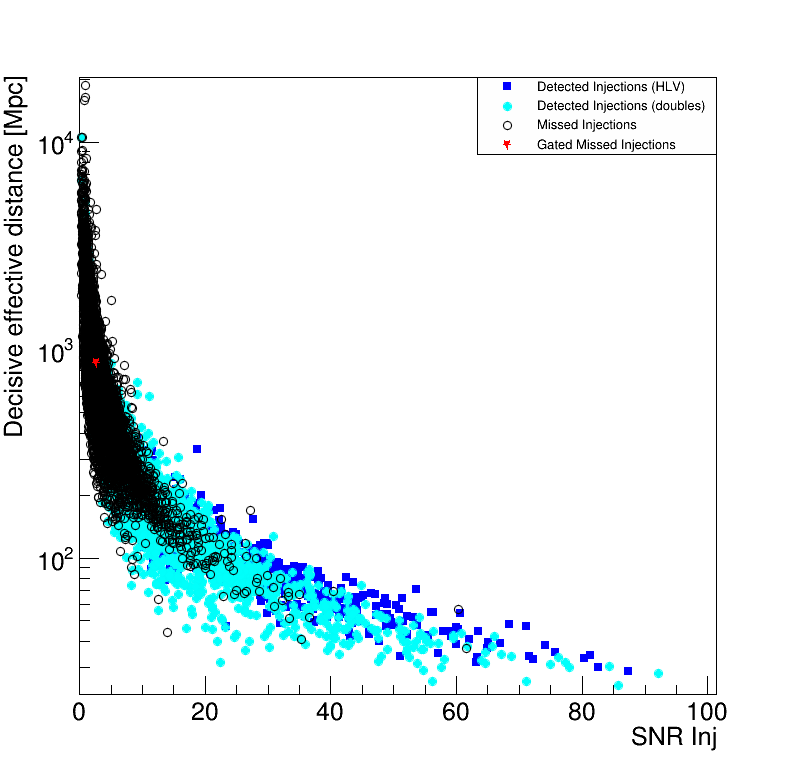
\includegraphics[width=0.5\linewidth]{sectionSelection/plotsOther/inj_recovery_snr_chunk26.png}
  \caption{Missed and found injections. Plots of the MBTA production monitoring for BNS injections on around 6 days.}
  \label{fig:injections_recovery}
\end{figure}
% \end{figure}


\begin{figure}
  \centering
  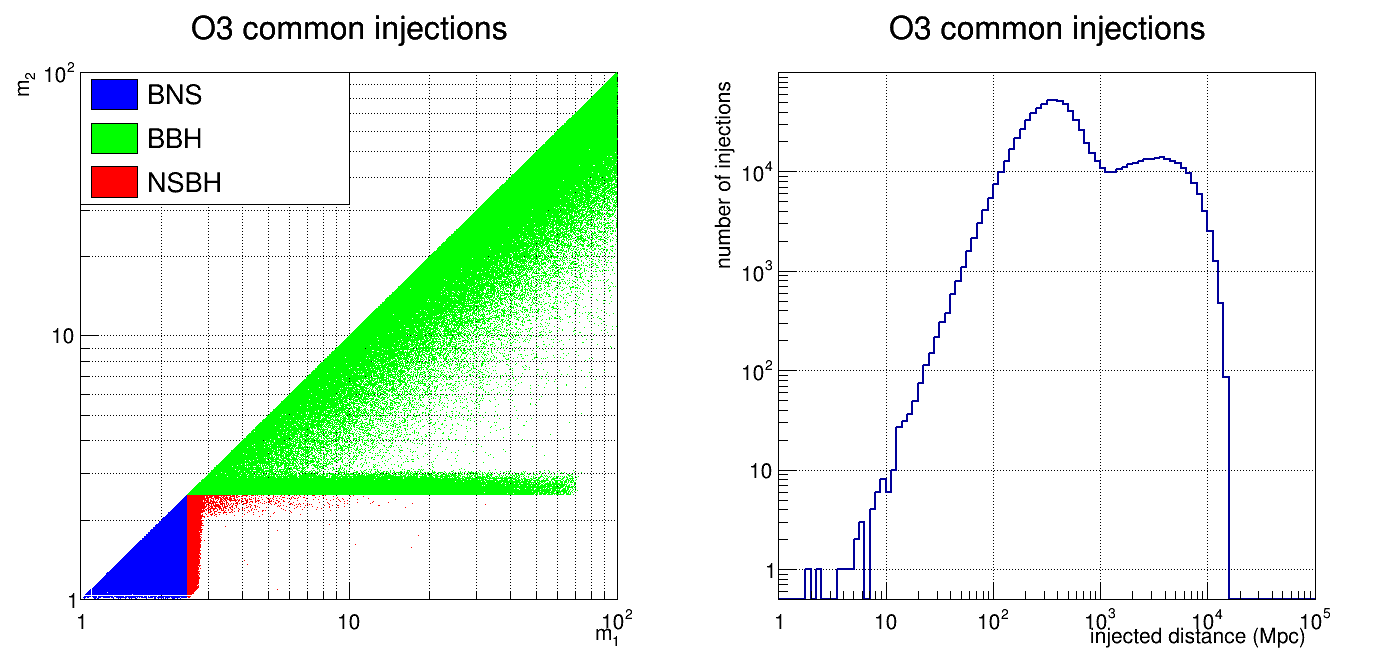
\includegraphics[width=\linewidth]{sectionSelection/plotsOther/cCommonInj.png}
  \caption{O3 common injections. Left: distribution of the masses for the injections. Right: distance distribution of the injections.}
  \label{fig:common_inj}
\end{figure}


%%%%%%%%%%
\clearpage\newpage
\subsection{Defining the EM bright population for single detector triggers}
\label{sec:embright}

We want to define a population of interest for the single detector trigger search.
This population, which we call EM bright, should contain most of the candidates susceptible of having an electromagnetic counterpart.
The most common process that is expected for the emission of EM waves is through the presence of a remnant mass \cite{bright_remnant}.
Thus it becomes natural to define this EM bright population according to the hasRemnant quantity computed by the pipeline (see section \ref{sec:pastro}).
To be safe we decide to consider as EM bright any candidate that has hasRemnant$>0.1\%$.
However the hasRemnant quantity was not computed for O3 injections as it was added after O3 catalogs were produced.
Therefore in this PhD work, we translate this definition in terms of just masses because the recovery of the spins is usually poor.
%  $\rightarrow$ Si hasRemnant: Since the study of single detector triggers had started before the developpment of the hasRemnant computation for single detector triggers I had to rely on a definition using the pipeline's parameter space, in fact only the masses because the recovery of the spins is too poor.}
Figures \ref{fig:m1_m2_hasRemnant} and \ref{fig:m1_mc_hasRemnant} show the hasRemnant value as a function of the individual masses and chirp mass for an injection run on 40 days of O3 replay data.

Based on these plots, we choose to define the EM bright population as follows:
% 
\begin{align}
  &\textrm{\SI{1}{\msun}} \leq m_1 \leq \textrm{\SI{50}{\msun}},\\
  &\textrm{\SI{1}{\msun}} \leq m_{chirp} \leq \textrm{\SI{5}{\msun}}
\end{align}
% 
which includes all recovered injections with hasRemnant$>0.1\%$.
We believe that this definition is conservative enough and should encompass more than just the EM bright candidates.
We use those constraints on the detected parameters as given above without concern for the effect of redshift since we do not expect high redshift for such sources.

Anything that is not part of this EM bright population is called EM dark.
%
\begin{figure}[hb]
  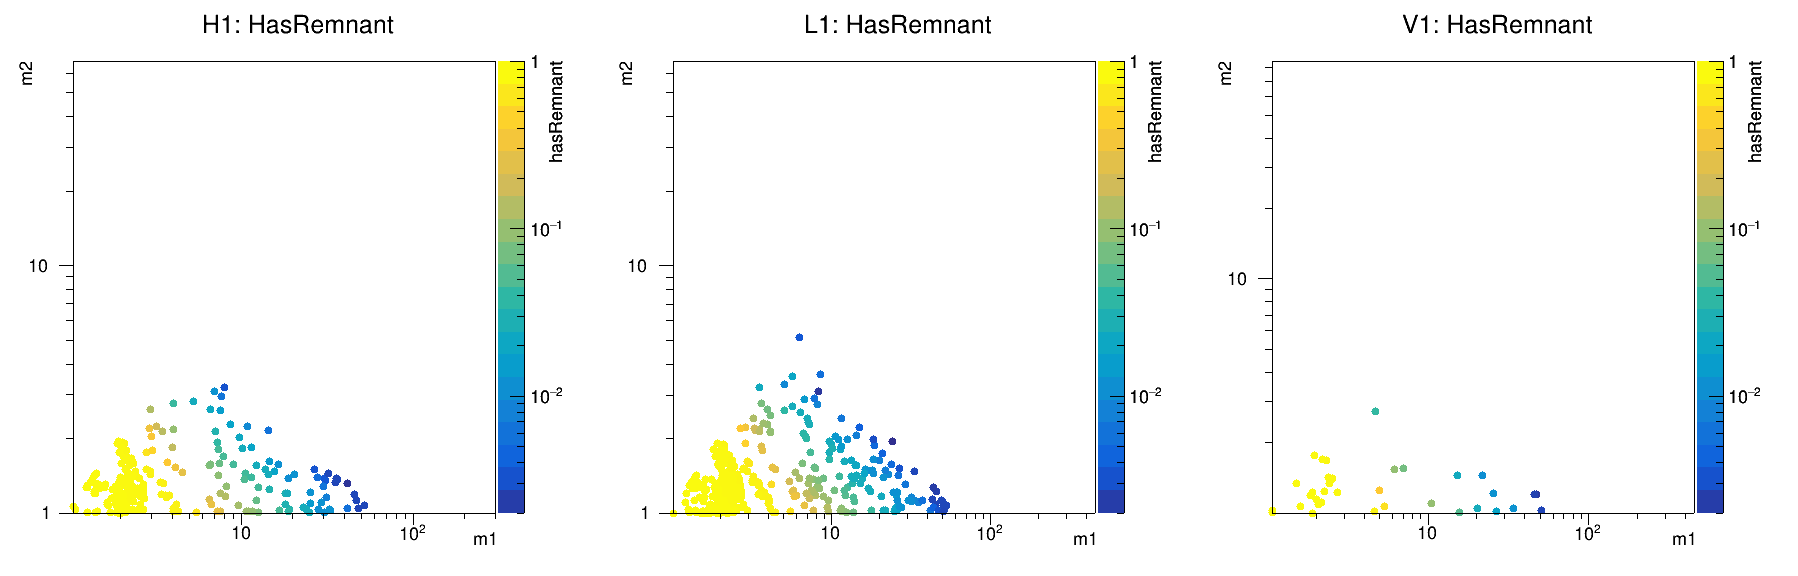
\includegraphics[width=\textwidth]{sectionSelection/plotsOther/embright_m1m2.png}
  \captionof{figure}{hasRemnant $>1\%$ versus $m_1$ and $m_2$ for single detector triggers during an injection run on O3 replay data.}
  \label{fig:m1_m2_hasRemnant}
\end{figure}
%
\begin{figure}[hb]
  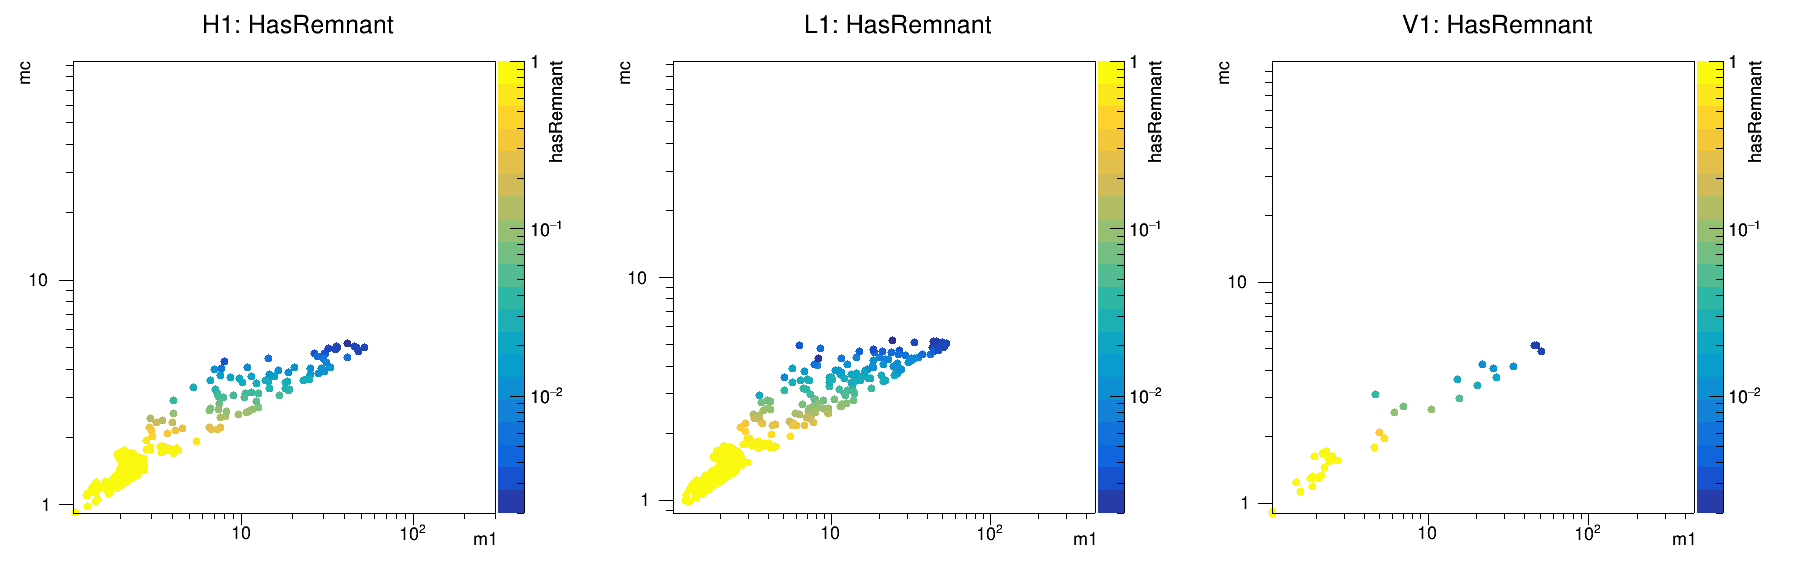
\includegraphics[width=\textwidth]{sectionSelection/plotsOther/embright_m1mc.png}
  \captionof{figure}{hasRemnant $>1\%$ versus $m_1$ and $m_{chirp}$ for single detector triggers during an injection run on O3 replay data.}
  \label{fig:m1_mc_hasRemnant}
\end{figure}



%%%%%%%%%% 
\clearpage\newpage
\subsection{Restraining the parameter space}
\label{sec:selec_param_space}

%{\large \textcolor{red}{Une fois la partie em bright/dark adapté la separation en embright/dark puis template duration ne devrait plus etre necessaire si la definition de EM bright est bien faite plus tot dans le manuscript}}

%\subsubsection{EM bright and dark populations}
%\label{sec:selec_embright}
%{\large \textcolor{red}{Adapter en fonction de comment la population a été introduite plus tot}}
%{\large \textcolor{red}{Mettre plot m1-m2-hasRemnant si pas mis avant?}}

%We define the EM bright population as follows, motivated by the LVC GRB paper \cite{paper_embright}:
% 
%\begin{align}
%  &\textrm{\SI{1}{\msun}} \leq m_1 \leq \textrm{\SI{25}{\msun}},\\
%  &\textrm{\SI{1}{\msun}} \leq m_2 \leq \textrm{\SI{2.8}{\msun}}
%\end{align}
% 
%The underlying idea is that we want at least 1 neutron star (matter) in the CBC system which imposes a small $m_2$ for the lightest object and either another neutron star or a small black hole such that tidal disruption is possible before the black hole swallows the neutron star.
%This requires a not-too-large $m_1$ for the heaviest object.
%The LVC GRB paper also considers constraints on the spins of the two objects but a study of parameter recovery on injected signals showed that the spins were badly recovered by MBTA, we therefore decided to not consider those constraints.
%Note that such a definition is very conservative and should encompass more than just the EM bright population.
%We use those constraints for our template bank parameter space as given above without concern for the effect of redshift since we do not expect high SNR sources at high red-shift values.
%Anything that is not part of this EM bright population is called EM dark.

%Figure \ref{fig:compare_bright_gaus} shows the distribution of O3 EM bright single detector triggers compared to Gaussian noise.
%\textcolor{red}{Getting ahead of ourselves we also show the comparison for long EM dark and short EM dark single detector triggers in figures \ref{fig:compare_longDark_gaus} and \ref{fig:compare_shortDark_gaus} respectively.
%Note that in the case of short EM dark triggers, the Gaussian noise did not produce many triggers because the region of the parameter space corresponding to this kind of signal is small.}


We want to focus on the EM bright triggers, as defined in section \ref{sec:embright} for the single detector triggers analysis.
% This is for two reasons: first because EM bright candidate are interesting for the astrophysics, second because due to the lower mass expected for those candidates their signal duration is longer.
% We expect glitches to mimic short signals which could trigger some short templates (this is especially relevant for BBH templates with high masses or sometimes high spins with duration that can be smaller than \SI{1}{s}).
% Adding to that the fact that the longer the signal the easier it is to identify (tools such as the \achi are not as efficient for very short template for instance) we can expect the background distribution for the EM bright triggers to be cleaner than for the EM dark candidates.
We show as a reference the background distribution for O3 singles detector triggers saved at all detector times in figure \ref{fig:O3_singles} (unlike figure \ref{fig:compare_bkg} which was for double and triple detector time only).
We easily verify that the EM bright population produces less noise triggers than the EM dark one by looking at the rwSNR distributions in figures \ref{fig:compare_bright_gaus} and \ref{fig:compare_dark_gaus}.

\begin{figure}[ht]
  \centering
  % O3 singles distribution
  \begin{minipage}{0.95\linewidth}
    \centering
    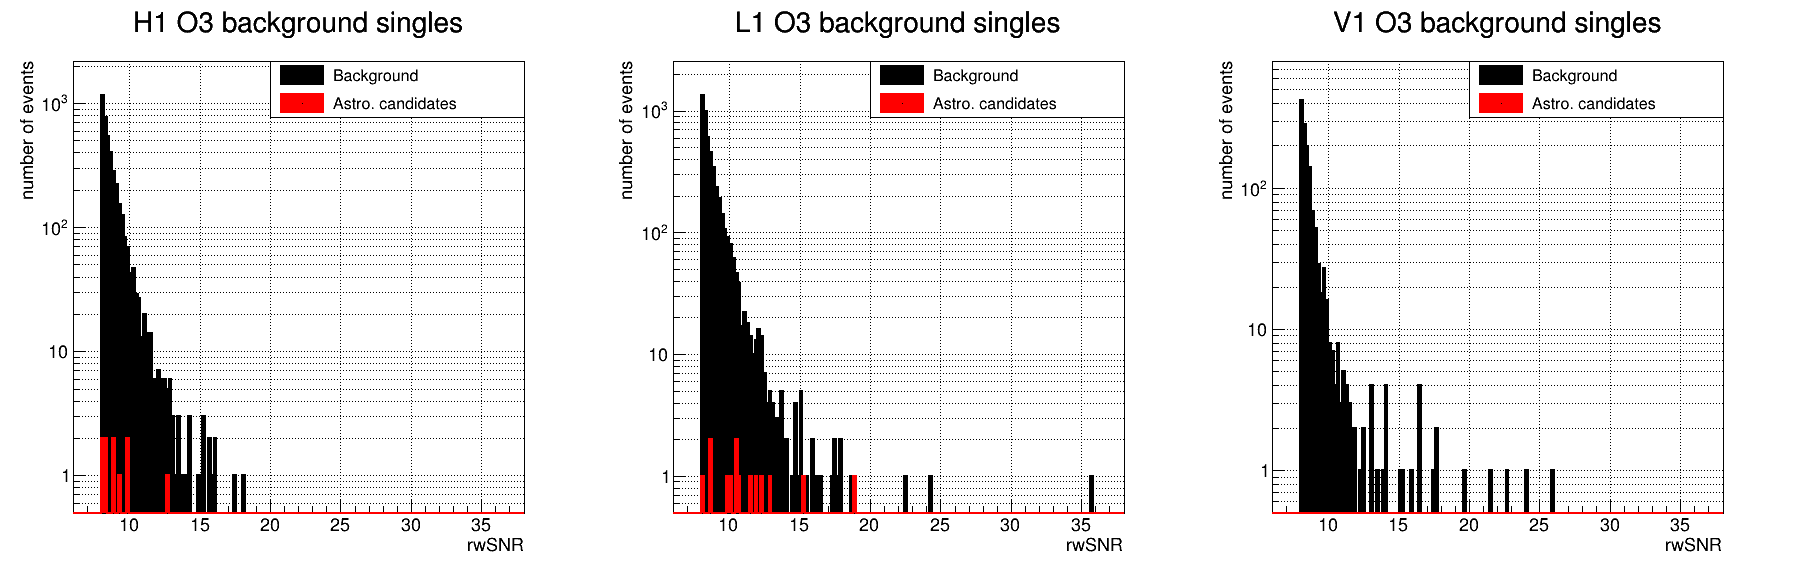
\includegraphics[width=\textwidth]{sectionSelection/plotsOther/cSinglesO3.png}
    \captionof{figure}{MBTA O3 single detector triggers from the offline analysis.}
    \label{fig:O3_singles}
  \end{minipage}
  \hfill
  \vspace{0.2cm}
  % 
  % EM bright vs Gaussian noise
  \begin{minipage}{0.95\linewidth}
    \centering
    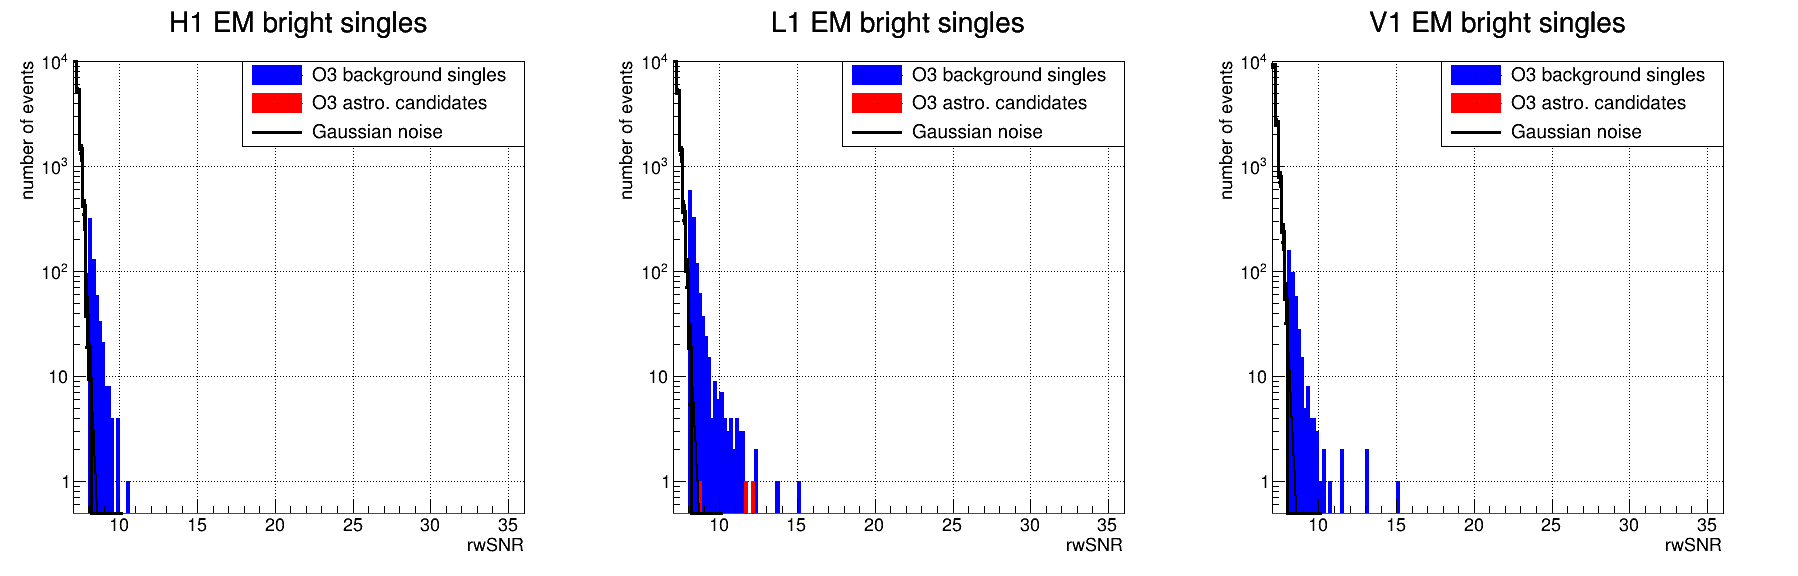
\includegraphics[width=\textwidth]{sectionSelection/plotsEMbright/cPosterNoCut.png}
    \captionof{figure}{rwSNR distribution for O3 EM bright single detector triggers before any specific single detector trigger selection.}
    \label{fig:compare_bright_gaus}
  \end{minipage}
  \hfill
  \vspace{0.2cm}
  % 
  % EM dark vs Gaussian noise
  \begin{minipage}{0.95\linewidth}
    \centering
    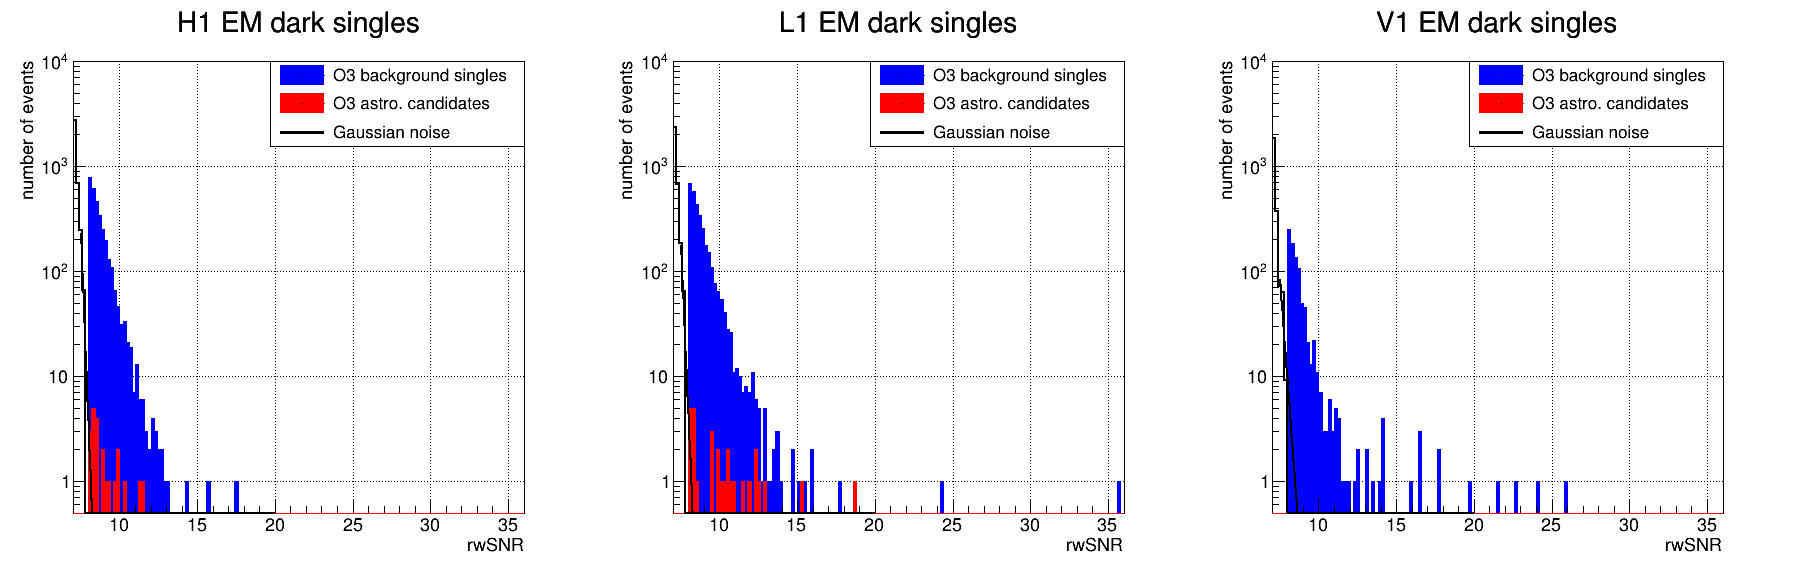
\includegraphics[width=\textwidth]{sectionSelection/plotsEMdark/cAllTemp.png}
    \captionof{figure}{rwSNR distribution for O3 EM dark single detector triggers before any specific single detector trigger selection.}
    \label{fig:compare_dark_gaus}
  \end{minipage}
  \hfill
\end{figure}
  
%\subsubsection{Selection using the template duration}
%\label{sec:selec_tempDur}


We know that we want to keep the EM bright candidates but we wonder whether we could also keep a part of the EM dark ones.
Since, as mentionned previously, the duration of the template may have an importance on the discrimination between noise and signal, we want to investigate this point.
Figure \ref{fig:singles_tempdur} shows, for each frequency bin, the number of single detector triggers saved during O3 divided by the number of template (O3 bank, all regions mixed).
The density of template as a function of the template duration is also shown.
We see that short templates produce way more triggers than the long ones.
Excluding such noisy templates from the single detector trigger search should therefore allow to reduce significantly the background.
We can go further with figures \ref{fig:embright_snrTempDur_nocut} and \ref{fig:emdark_snrTempDur_nocut}.
They show respectively the distribution of EM bright and EM dark single detector triggers in the rwSNR versus template duration plane and confirm that EM bright templates are generally longer.
We have therefore no reason to split the EM bright population based on the template duration.
EM dark templates however exhibit many triggers with short duration and large rwSNR.
What appear as vertical lines in figure \ref{fig:emdark_snrTempDur_nocut} are very noisy templates which produce many triggers.
To exclude these triggers we decide to split the EM dark population in a ``long EM dark'' population with template duration $\geq$ \SI{0.8}{s} and a ``short EM dark'' population with template duration $<$ \SI{0.8}{s}.


\begin{figure}[hb]
  \centering
  \begin{minipage}{0.45\linewidth}
    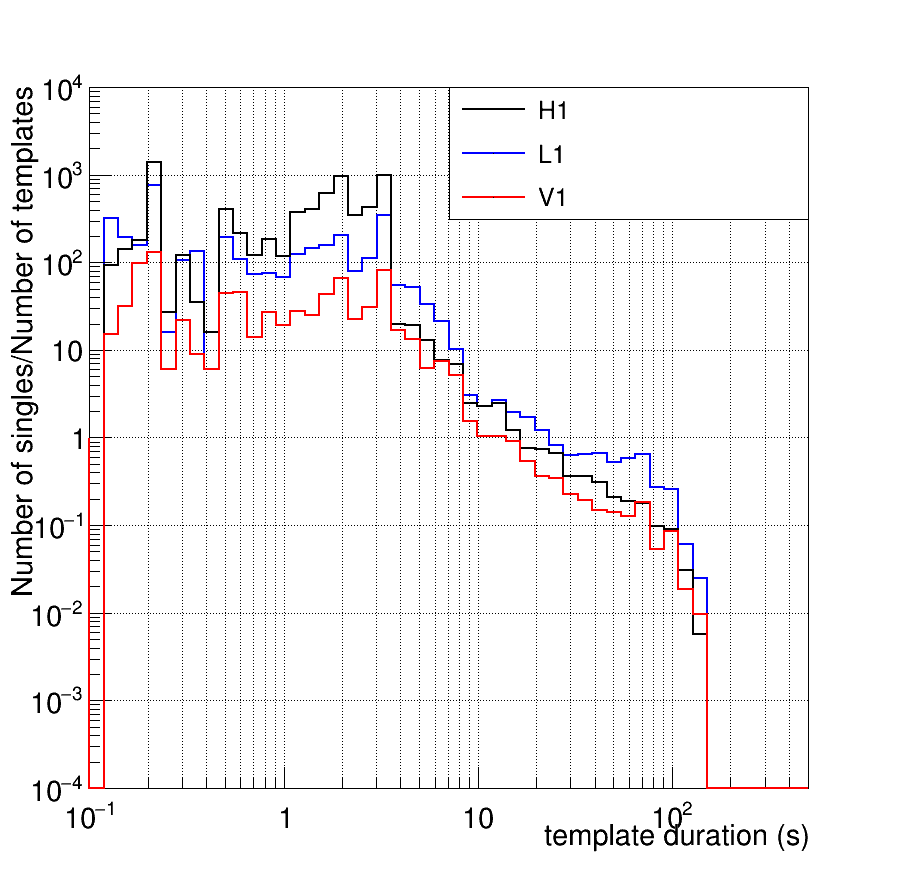
\includegraphics[width=\textwidth]{sectionSelection/plotsOther/cDurationSingles.png}
  \end{minipage}
  \hfill
  \begin{minipage}{0.45\linewidth}
    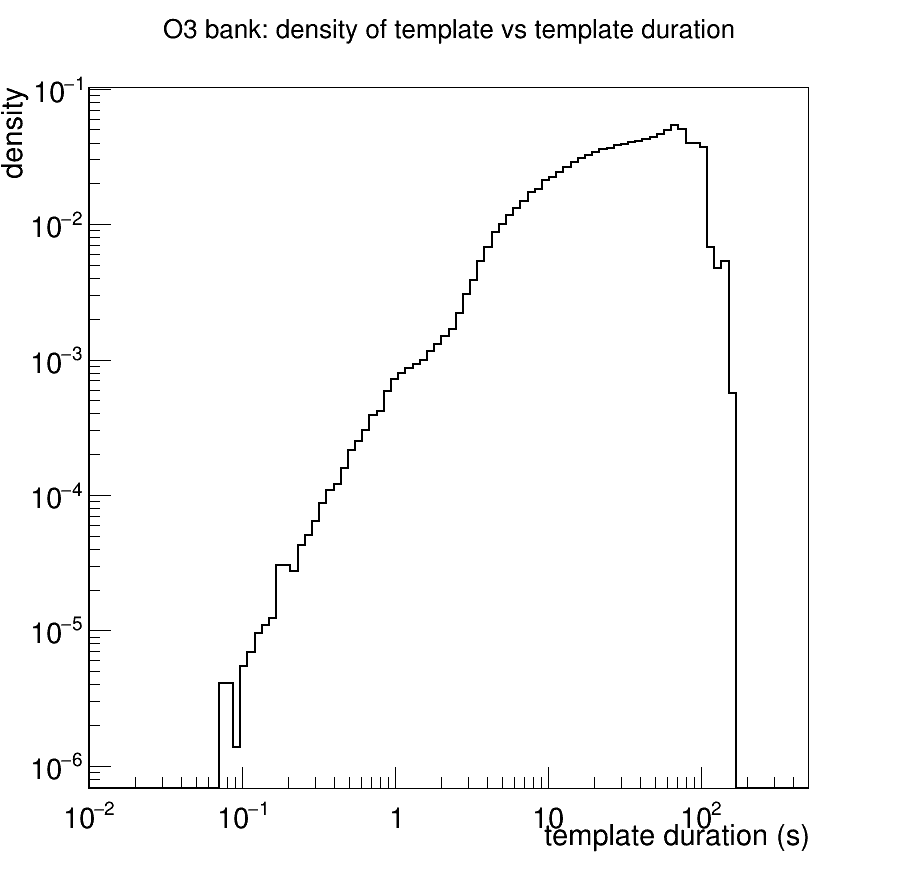
\includegraphics[width=\textwidth]{sectionSelection/plotsOther/cTempDensity.png}
  \end{minipage}    
  \caption{Left: Number of MBTA O3 single detector triggers per template as a function of the template duration. Right: Density of templates (number of templates per bin relative to the total number of templates) as a function of the template duration for MBTA's O3 template bank.}
  \label{fig:singles_tempdur}
\end{figure}

% EM BRIGHT TEMPLATE DURATION PLOTS
%
\begin{figure}[hb]
  \centering
  \begin{minipage}{0.95\linewidth}
    \centering
    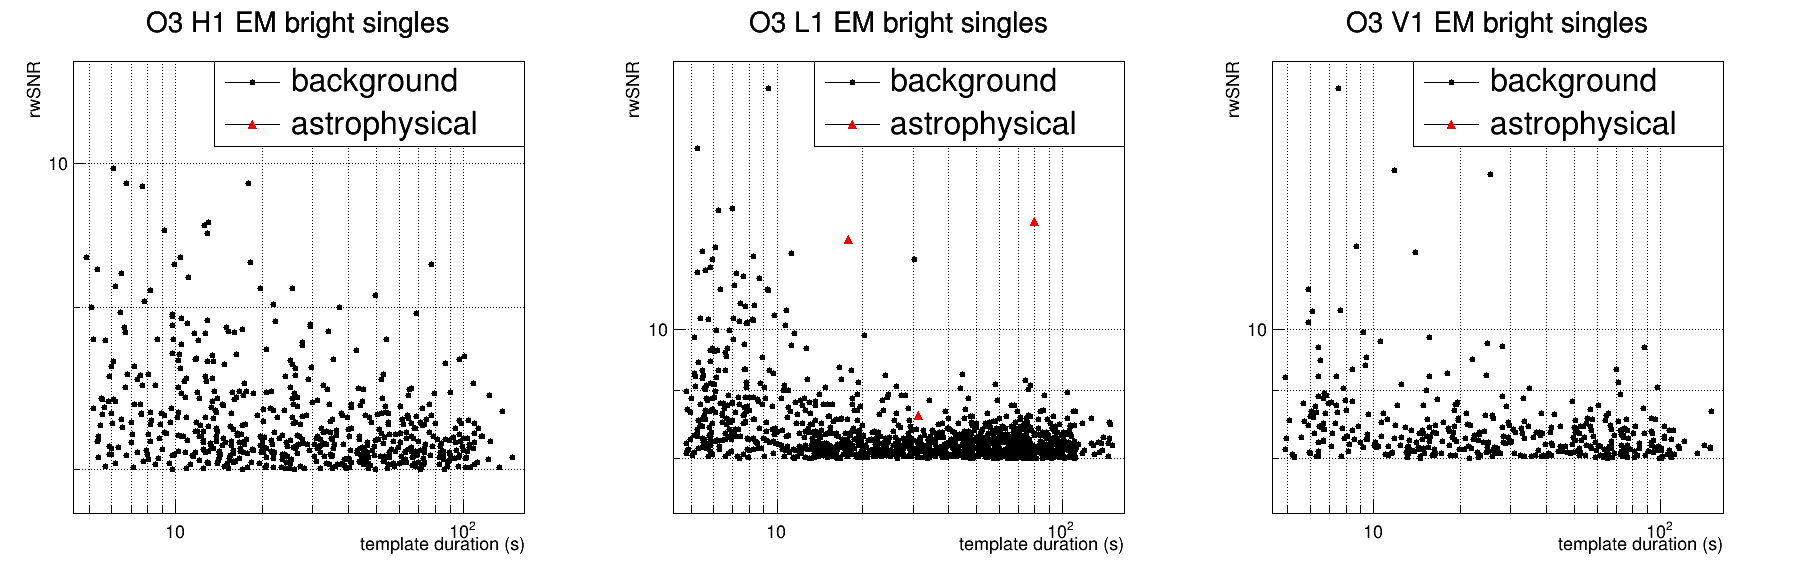
\includegraphics[width=\linewidth]{sectionSelection/plotsEMbright/cSnrTempDur.png}
    \captionof{figure}{Distribution of the O3 EM bright single detector triggers in the template duration vs rwSNR plane.}
    \label{fig:embright_snrTempDur_nocut}
  \end{minipage}
  \hfill
%%
%
% EM DARK TEMPLATE DURATION PLOTS
%% 
  \begin{minipage}{0.95\linewidth}
    \centering
    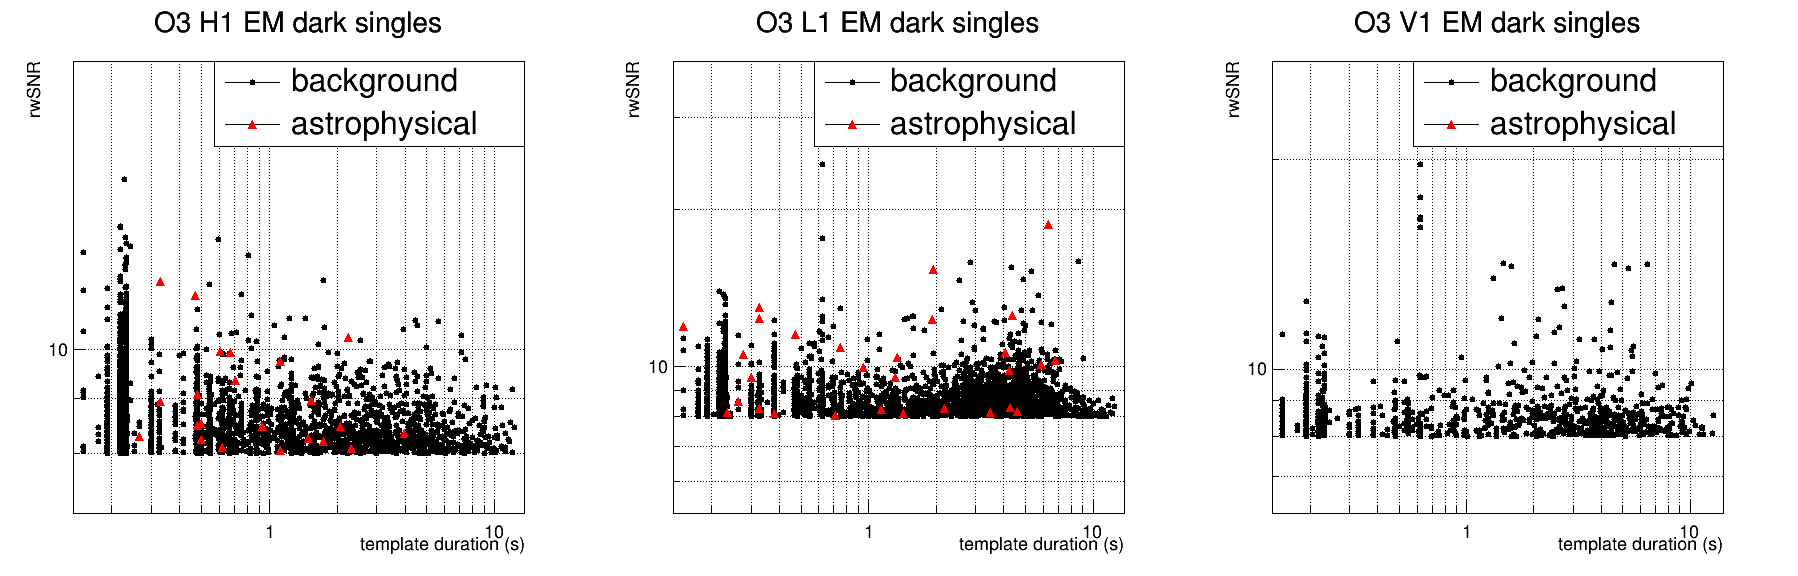
\includegraphics[width=\linewidth]{sectionSelection/plotsEMdark/cSnrTempDur.png}
    \captionof{figure}{Distribution of the O3 EM dark single detector triggers in the template duration vs rwSNR plane. A few short templates are triggered very often, showing as vertical lines.}
    \label{fig:emdark_snrTempDur_nocut}
  \end{minipage}
  \hfill
\end{figure}
%%
%% 

% % EM BRIGHT CUT DURATION PLOTS
% \begin{figure}
%   \centering
%   \begin{minipage}{0.45\linewidth}
%     \centering
%     \includegraphics[width=\linewidth]{SingleSelection/EMbright/cCumH1_tempdur.png}
%     \captionof{figure}{Cumulative rwSNR distribution of H1 background EM bright singles for various cuts on the template duration (the cut on the excess rate is applied).}
%     \label{fig:cut_tempdur_embright_H1}
%   \end{minipage}
%   \hfill
%   % 
%   \begin{minipage}{0.45\linewidth}
%     \centering
%     \includegraphics[width=\linewidth]{SingleSelection/EMbright/cCumL1_tempdur.png}
%     \captionof{figure}{Cumulative rwSNR distribution of L1 background EM bright singles for various cuts on the template duration (the cut on the excess rate is applied).}
%     \label{fig:cut_tempdur_embright_L1}
%   \end{minipage}
%   \hfill
%   \vspace{5mm}
%   % 
%   \begin{minipage}{0.45\linewidth}
%     \centering
%     \includegraphics[width=\linewidth]{SingleSelection/EMbright/cCumV1_tempdur.png}
%     \captionof{figure}{Cumulative rwSNR distribution of V1 background EM bright singles for various cuts on the template duration (the cut on the excess rate is applied).}
%     \label{fig:cut_tempdur_embright_V1}
%   \end{minipage}
%   \hfill
% \end{figure}
% %%
% %%
% % EM DARK CUT DURATION PLOTS
% \begin{figure}
%   \centering
%   \begin{minipage}{0.45\linewidth}
%     \centering
%     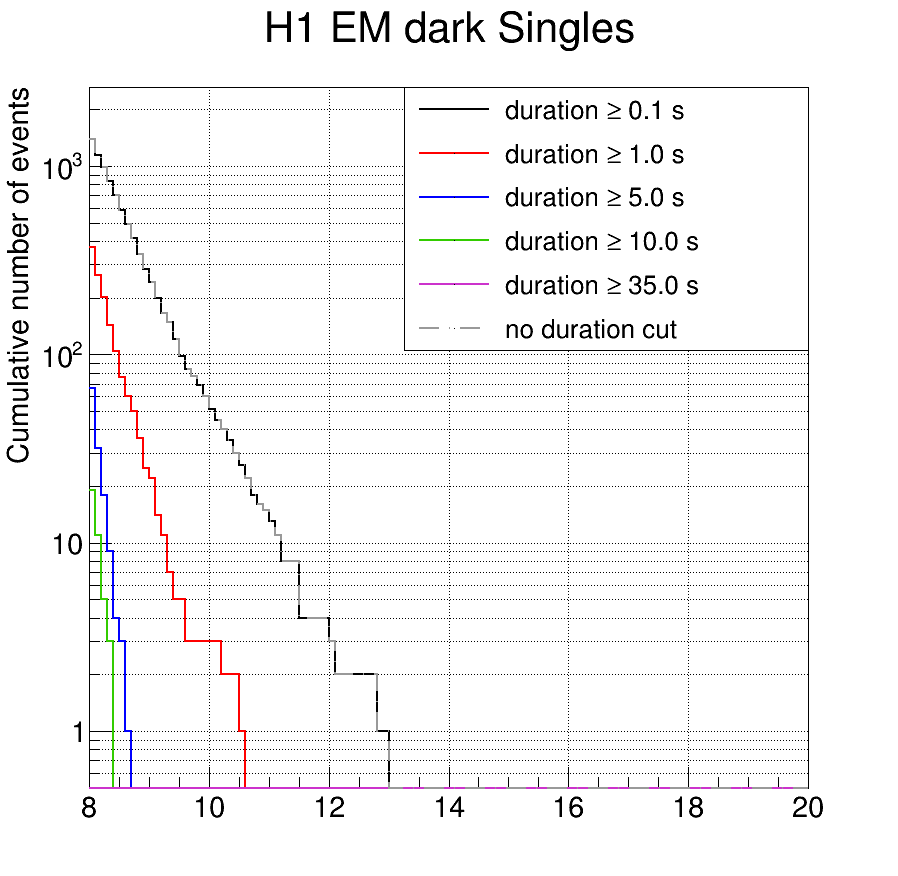
\includegraphics[width=\linewidth]{SingleSelection/EMdark/cCumH1_tempdur_ermax.png}
%     \captionof{figure}{Cumulative rwSNR distribution of H1 background EM dark singles for various cuts on the template duration (the cuts on the gating and excess rate are applied).}
%     \label{fig:cut_tempdur_emdark_H1}
%   \end{minipage}
%   \hfill
%   % 
%   \begin{minipage}{0.45\linewidth}
%     \centering
%     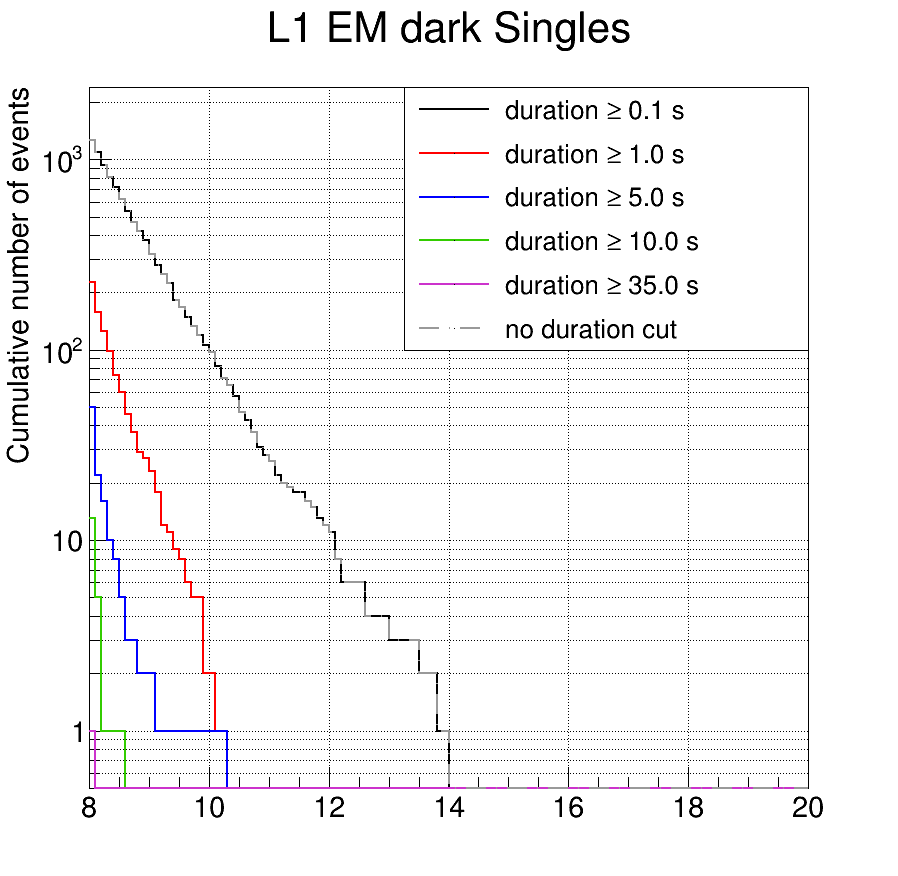
\includegraphics[width=\linewidth]{SingleSelection/EMdark/cCumL1_tempdur_ermax.png}
%     \captionof{figure}{Cumulative rwSNR distribution of L1 background EM dark singles for various cuts on the template duration (the cuts on the gating and excess rate are applied).}
%     \label{fig:cut_tempdur_emdark_L1}
%   \end{minipage}
%   \hfill
%   \vspace{5mm}
%   % 
%   \begin{minipage}{0.45\linewidth}
%     \centering
%     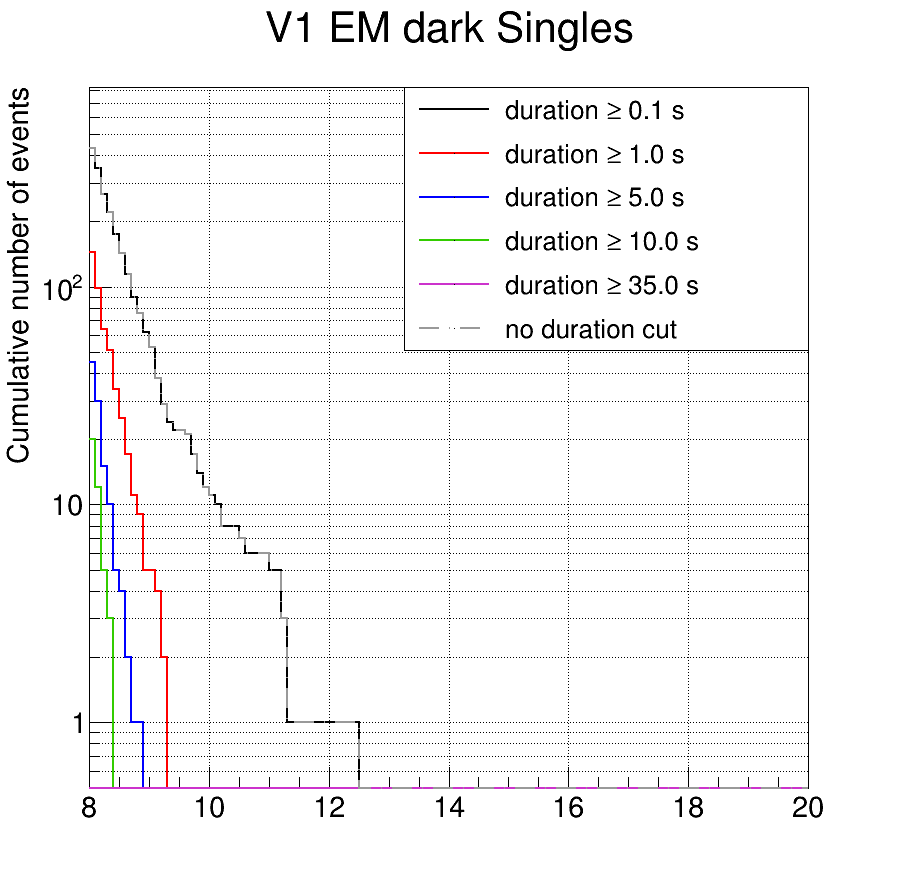
\includegraphics[width=\linewidth]{SingleSelection/EMdark/cCumV1_tempdur_ermax.png}
%     \captionof{figure}{Cumulative rwSNR distribution of V1 background EM dark singles for various cuts on the template duration (the cuts on the gating and excess rate are applied).}
%     \label{fig:cut_tempdur_emdark_V1}
%   \end{minipage}
%   \hfill
% \end{figure}
% %% 
% %% 
% % long EM dark vs Gaussian noise
% \begin{figure}
%   \centering
%   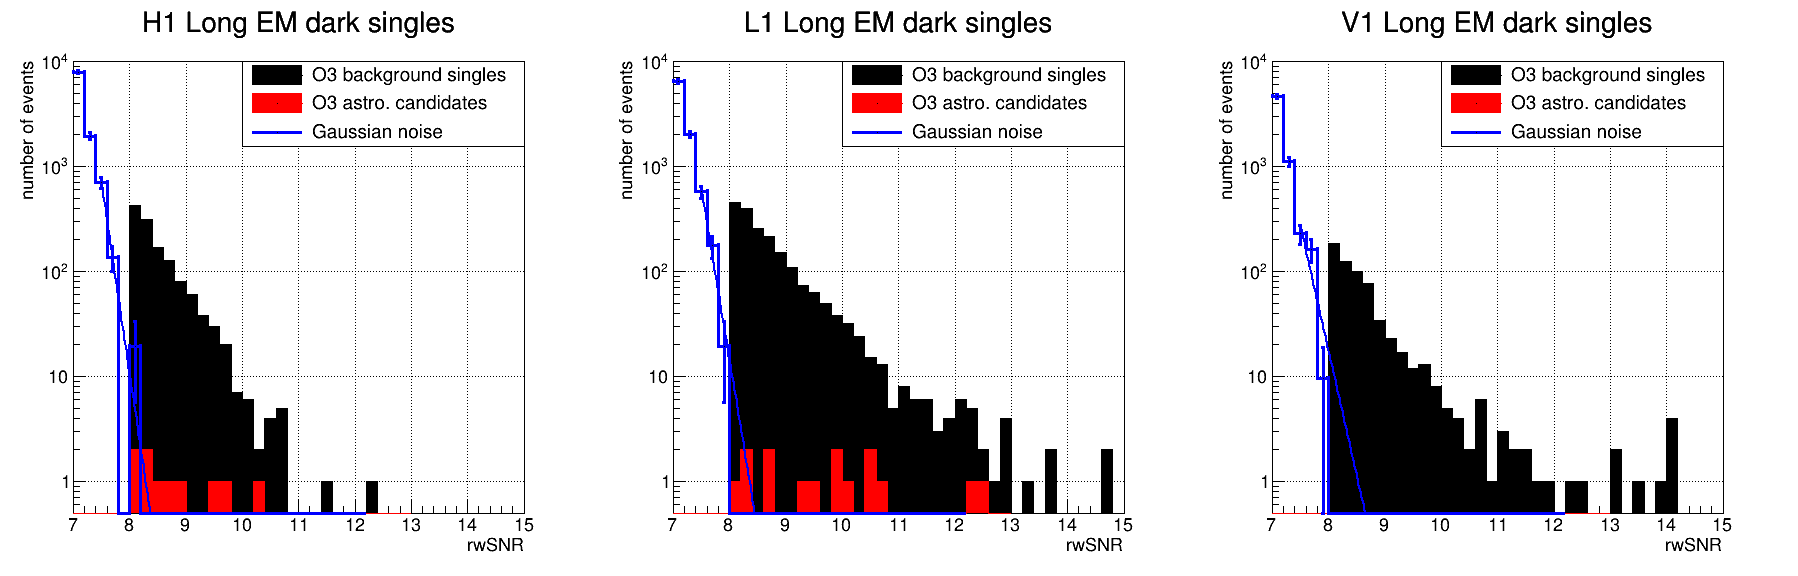
\includegraphics[width=\textwidth]{SingleSelection/EMdark/cPosterDarkLong_noCut.png}
%   \caption{Long EM dark single detector triggers: O3 before selection vs Gaussian noise (4 chunks scaled to the total observation time of O3)}
%   \label{fig:compare_longDark_gaus}
% \end{figure}

% % short EM dark vs Gaussian noise
% \begin{figure}
%   \centering
%   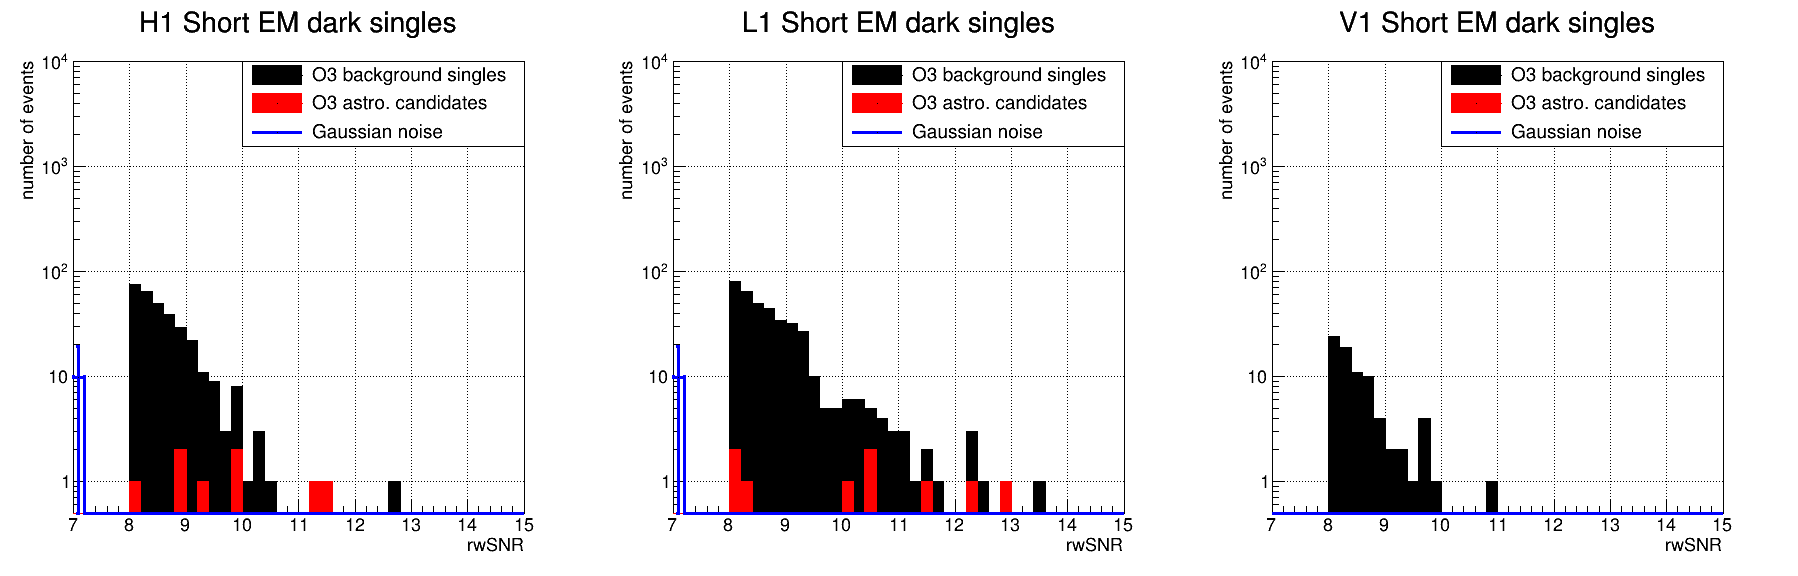
\includegraphics[width=\textwidth]{SingleSelection/EMdark/cPosterDarkShort_noCut.png}
%   \caption{Short EM dark single detector triggers: O3 before selection vs Gaussian noise (4 chunks scaled to the total observation time of O3)}
%   \label{fig:compare_shortDark_gaus}
% \end{figure}
%% 
%% 



%%%%%%%%%% 
\clearpage\newpage
\subsection{Selection using the \texorpdfstring{\achi}{autoChi2}}
\label{sec:selec_autochi2}
The first quantity we consider to define specific single detector trigger selection criteria is the \achi.
It is already used to computed the reweighted SNR but does not remove all noise triggers and relies on coincidences to clean what is left.
Here we want something more powerful even at the cost of some loss of duty cycle.
We therefore decide to investigate a cut on the \achi.

There are no physical motivations to choose a specific cut value, but we know that the \achi has a tendency to grow with the SNR.
The cut should therefore take this into account to avoid rejecting loud astrophysical signals.
We use a set of injections to choose a cut that allows to reject background triggers while only removing at most a few percent of the injections.
The tentative cut is the following:
%
\begin{equation}
    \text{auto}\chi^2 \leq 2+0.005 \times \text{SNR}^2
\end{equation}
%
The quadratic dependence in the SNR is motivated by the formula of the \achi.
More details about this SNR dependence of the \achi are given in section \ref{sec:snr_dependency}.
This dependence should not change from one O3 region of the parameter space to the other since the banks are made with the same minimal match parameter.
This cut is therefore tested for the three regions all together.

The corresponding threshold is shown in figure \ref{fig:inj_achi2}, drawn over the distribution of recovered BBH injections in the plane \achi vs SNR.
The fractions of astrophysical injections surviving the cut in the 3 regions are given in table \ref{tab:inj_frac}.
%
\begin{table}[h]
    \centering
    \begin{tabular}{c|c|c|c}
         & H1 & L1 & V1 \\ \hline
         BNS & 0.999 & 0.995 & 0.995 \\
         BBH & 0.980 & 0.954 & 0.997 \\
         NSBH & 0.982 & 0.974 & 0.982 \\
    \end{tabular}
    \caption{Fraction of injections surviving the \achi cut for each search region and detector.}
    \label{tab:inj_frac}
\end{table}
%
When taking this cut and applying it to O3 EM bright singles it turns out that none of them falls outside of the acceptable (SNR, \achi) values as shown by figure \ref{fig:achi2_bright}.
EM dark single detector triggers are barely affected and the tail of their rwSNR distribution is unchanged.
As can be seen on figure \ref{fig:inj_achi2}, a more aggressive cut would start removing astrophysical signals.
This cut is therefore not considered further.

\begin{figure}[hb]
    \centering
    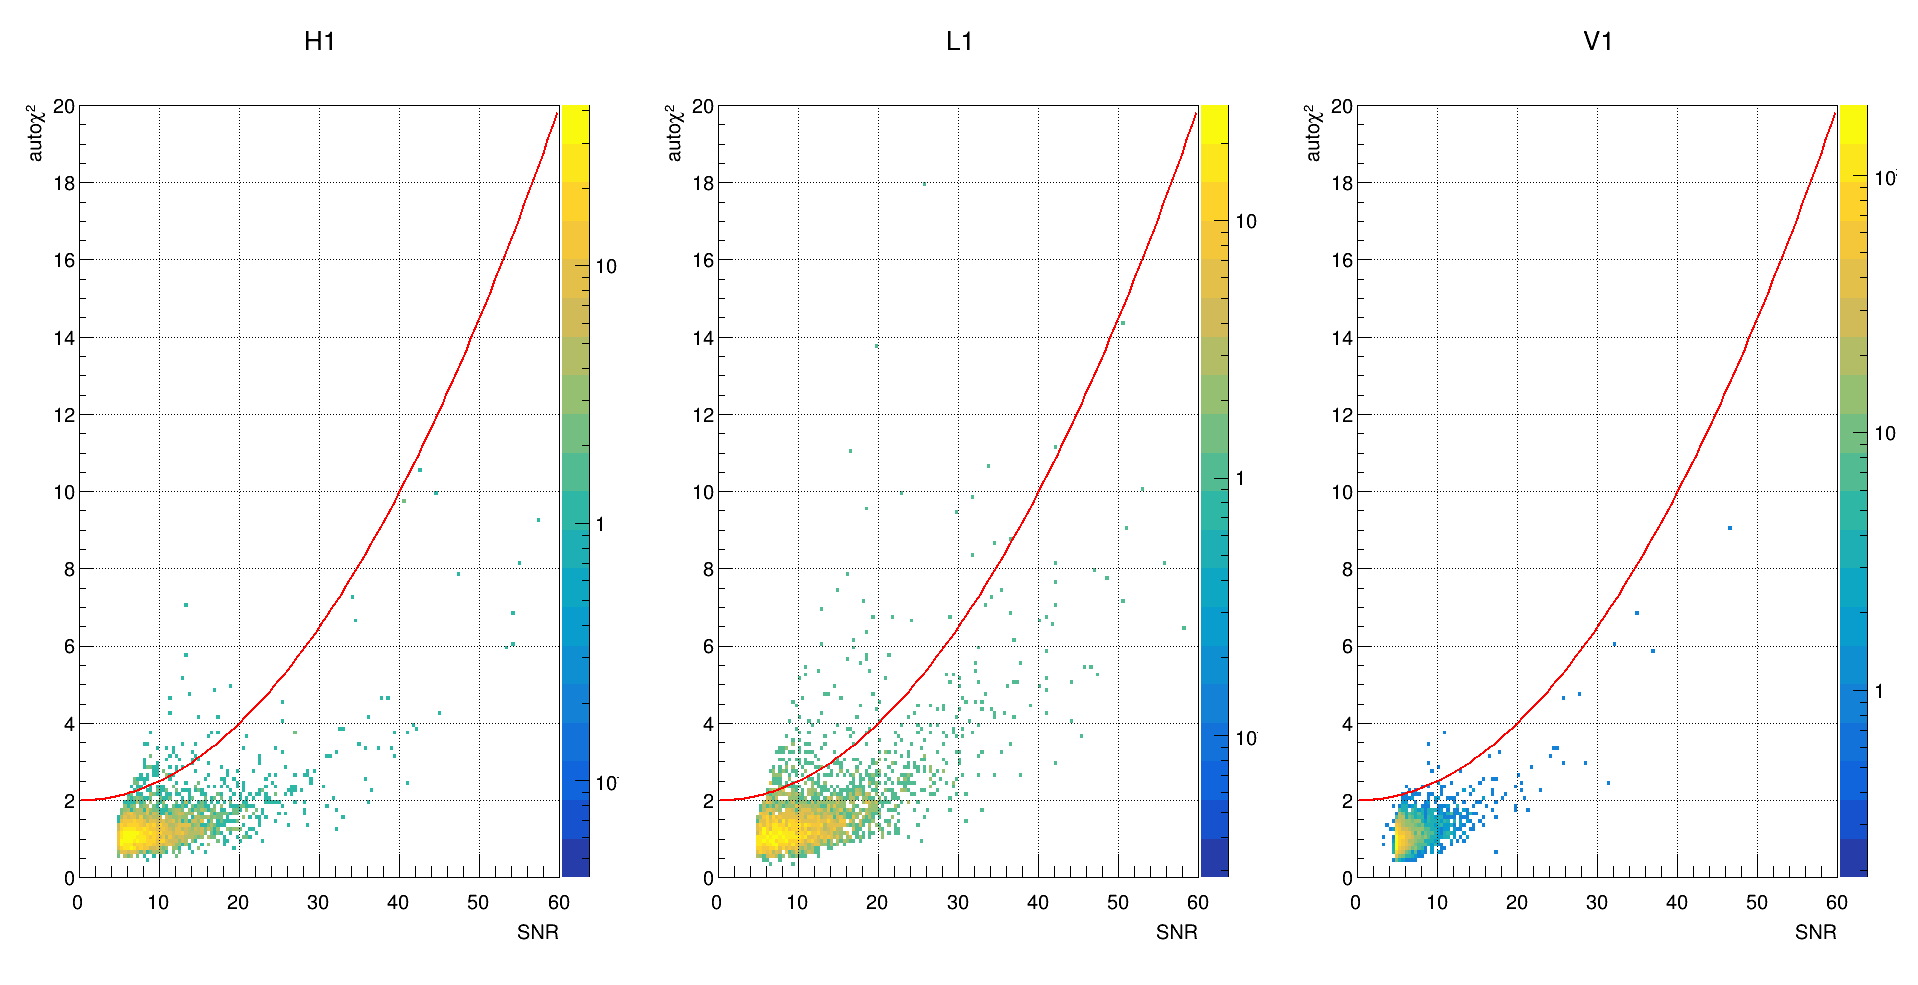
\includegraphics[width=\textwidth]{sectionSelection/plotsOther/cSnrAchi2InjCut_BBH.png}
    \caption{BBH injections distribution in the \achi vs SNR plane. The tentative threshold chosen for the cut is drawn in red: anything above the line is rejected.}
    \label{fig:inj_achi2}
\end{figure}

\begin{figure}[hb]
    \centering
    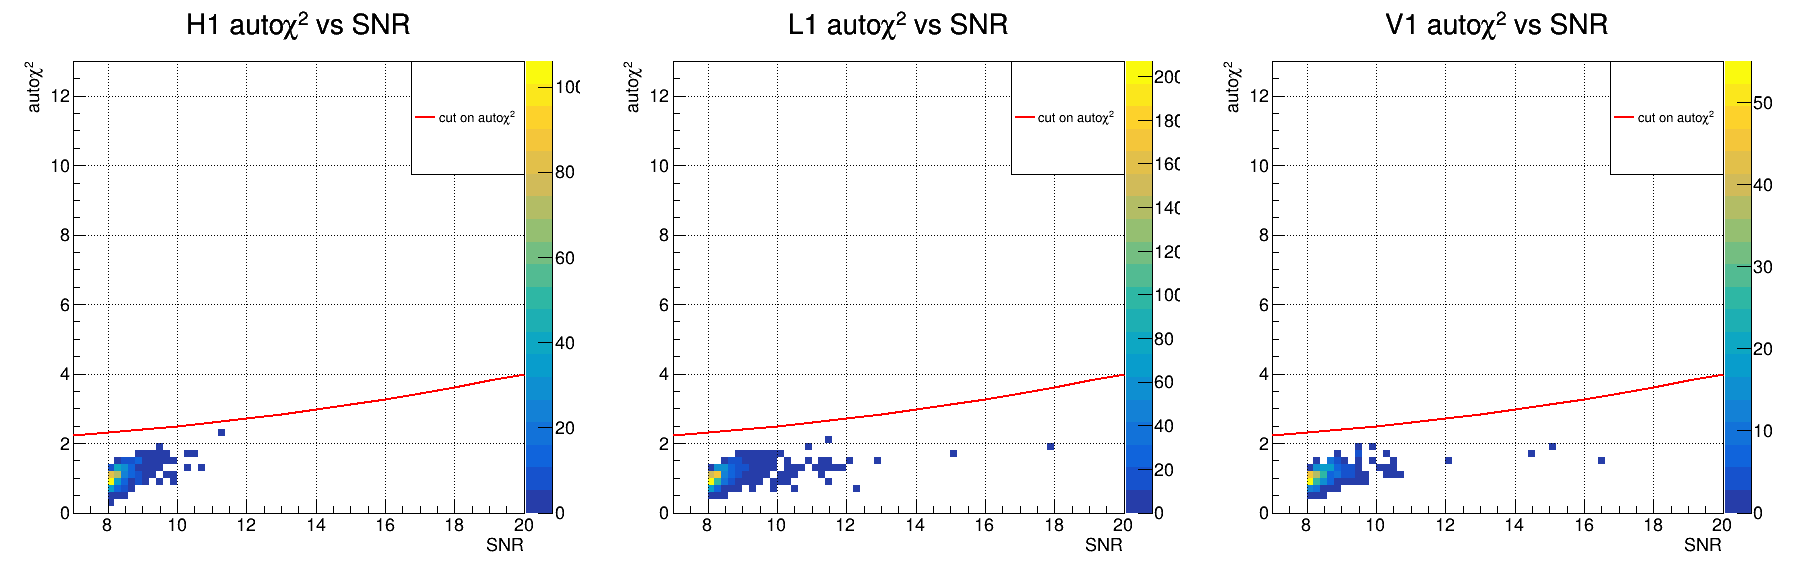
\includegraphics[width=\textwidth]{sectionSelection/plotsEMbright/cCutAchi2Bright.png}
    \caption{O3 EM bright single detector triggers distribution in the \achi vs SNR plane. The tentative threshold chosen for the cut is drawn in red: anything above the line is rejected.}
    \label{fig:achi2_bright}
\end{figure}



%%%%%%%%%% 
\clearpage\newpage
\subsection{Selection using the excess rate}
\label{sec:selecER}

The second quantity we consider to define selection criteria is the excess rate (ER).
We want to reject triggers that were detected during bad data quality times and this is exactly what the ER is telling us.
Our approach is straightforward: we want to define a threshold on the ER above which candidates will be rejected.
Reweighting the SNR as for the coincidences could work but very loud noise triggers could still be quite significant after reweighting.
We therefore choose to apply a cut to be on the safe side.

\subsubsection{Which excess rate should we use?}
\label{sec:correl_ER}
There were 3 types of ER during O3, one for each search region (BNS, BBH, NSBH) but this will not be the case for O4 anymore.
We can show (figure \ref{fig:correl_erw}) that the different ER are correlated.
Since we want to find a cut value for these excess rates that would allow to reduce the tail of the background SNR distribution, this correlation is a good argument to be even more restrictive by cutting on the maximum of the three excess rates.
%% 

\begin{figure}[hb]
  \centering
  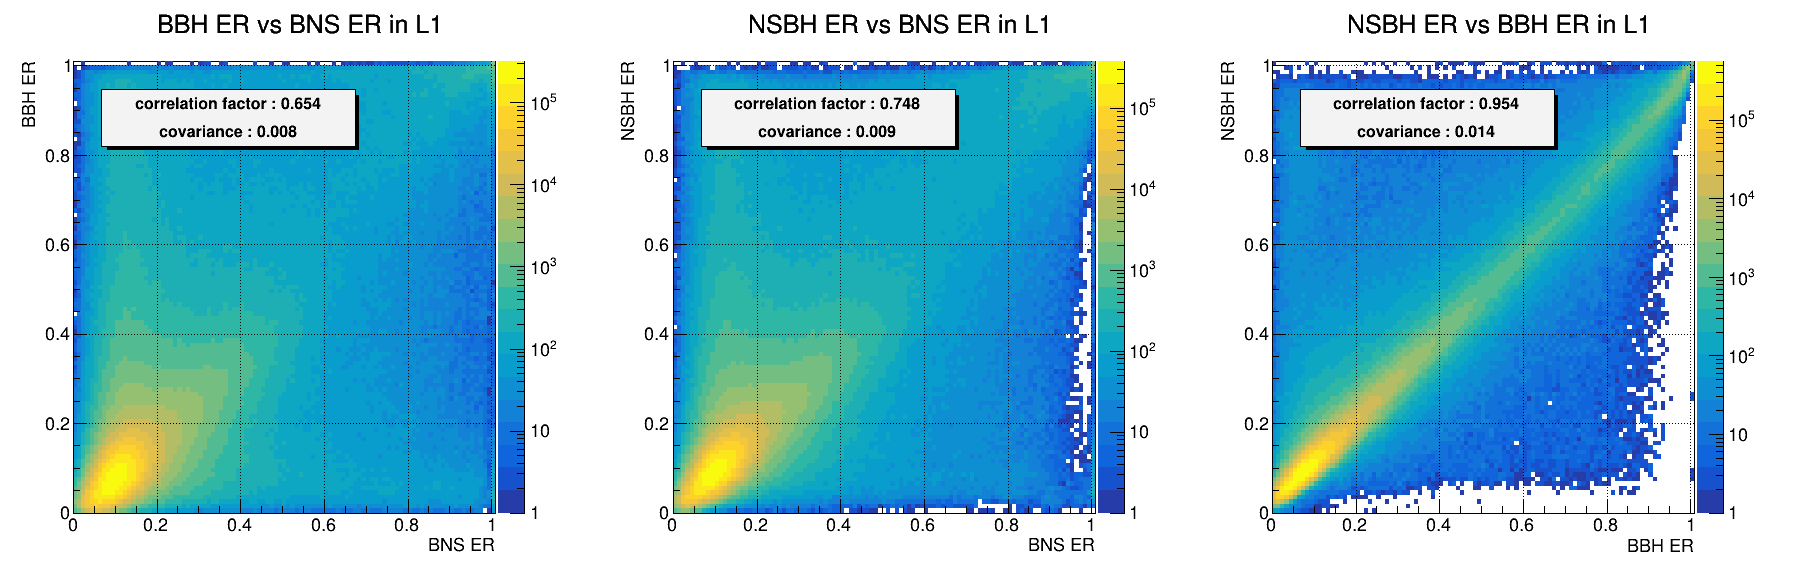
\includegraphics[width=\textwidth]{sectionSelection/plotsOther/correlERL1.png}
  \caption{Pairwise comparison of the 3 types of excess rates observed during O3 in L1. Correlations factor greater than 0.5 indicate strong correlation between the different ER. The correlation factor is the covariance of the excess rates divided by the product of their standard deviation.}
  \label{fig:correl_erw}
\end{figure}



\subsubsection{Excess rate on EM bright single detector triggers}
\label{sec:embright_er}

Figure \ref{fig:cut_erw_embright} shows the effect of a cut rejecting all background trigger at times with $\text{ER}>0.3$ on the EM bright SNR distribution for the 3 excess rates and their maximum.
All confirmed candidates published in the GWTC-2.1 \cite{gwtc2.1} and GWTC-3 \cite{gwtc3} catalogues were removed.
The maximum ER gives by construction the best result with only few SNR values above 9 and does not reject much more duty cycle than the others, which comforts us in choosing it to apply a cut.

The value of $\text{ER}=0.3$ for the cut is equal to the threshold used to reweight the SNR with the excess rate for coincidences.
Softer values of cut did not clean as well the SNR distribution.
Using a harsher cut would reduce even more the duty cycle while not removing much more background triggers as shown by figure \ref{fig:embright_ercut}.
Thus we settle for a cut at $\textrm{ER}=0.3$.
But this will have to be checked again with O4 noise.

Figure \ref{fig:embright_astro_ercut} shows the effect of the cut on the EM bright background along the astrophysical candidates given in table \ref{tab:astro} (with parameter within the EM bright region, coming from the GWTC2.1 \cite{gwtc2.1} and GWTC3 catalogs \cite{gwtc3}).
Plots are only shown for L1 because it is the most sensitive out of the three detectors and the only one in which we have single detector triggers from EM bright astrophysical signals.
We see that we have rejected many triggers at high rwSNR but the astrophysical signals, although not impacted by the cut, still do not stand out of the distribution because of a few significant background triggers remaining.
%% 
% \begin{figure}[hb]
%   \centering
%   \begin{minipage}{0.45\linewidth}
%     \centering
%     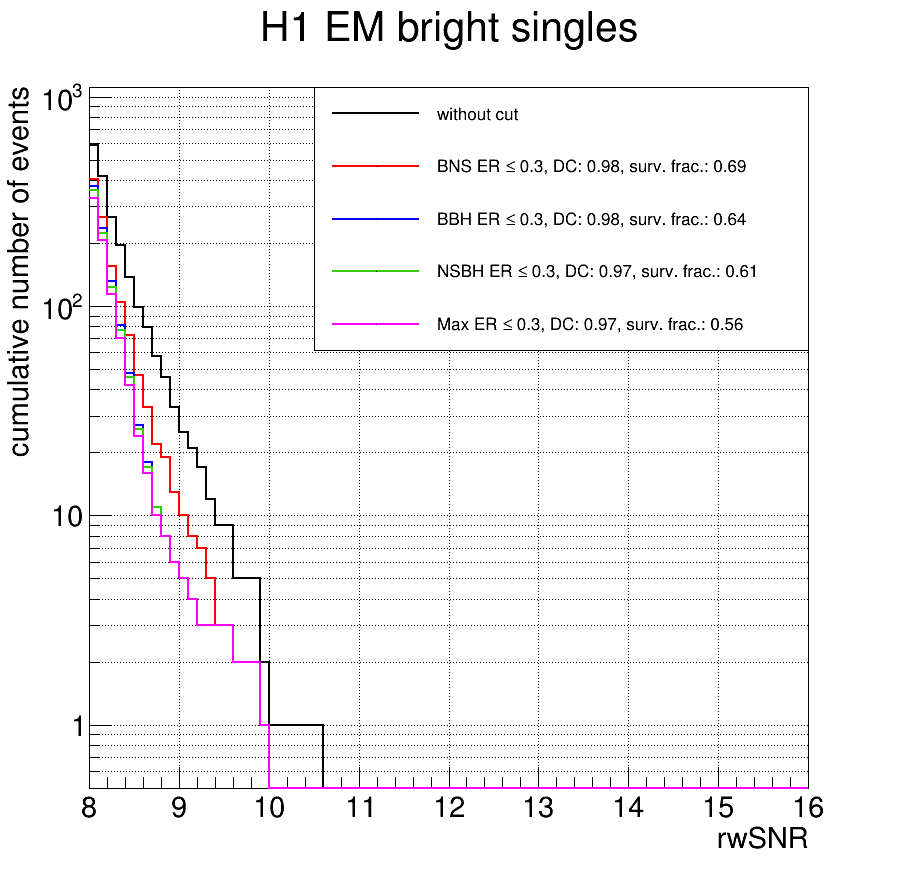
\includegraphics[width=\linewidth]{sectionSelection/plotsEMbright/cCumH1_er.png}
%     \captionof{figure}{Cumulative rwSNR distribution of O3 H1 background EM bright single detector triggers for various cuts on the excess rate. The legend also indicates in each case the remaining duty cycle (DC) and surviving fraction of single detector triggers.}
%     \label{fig:cut_erw_embright_H1}
%   \end{minipage}
%   \hfill
%   % 
%   \begin{minipage}{0.45\linewidth}
%     \centering
%     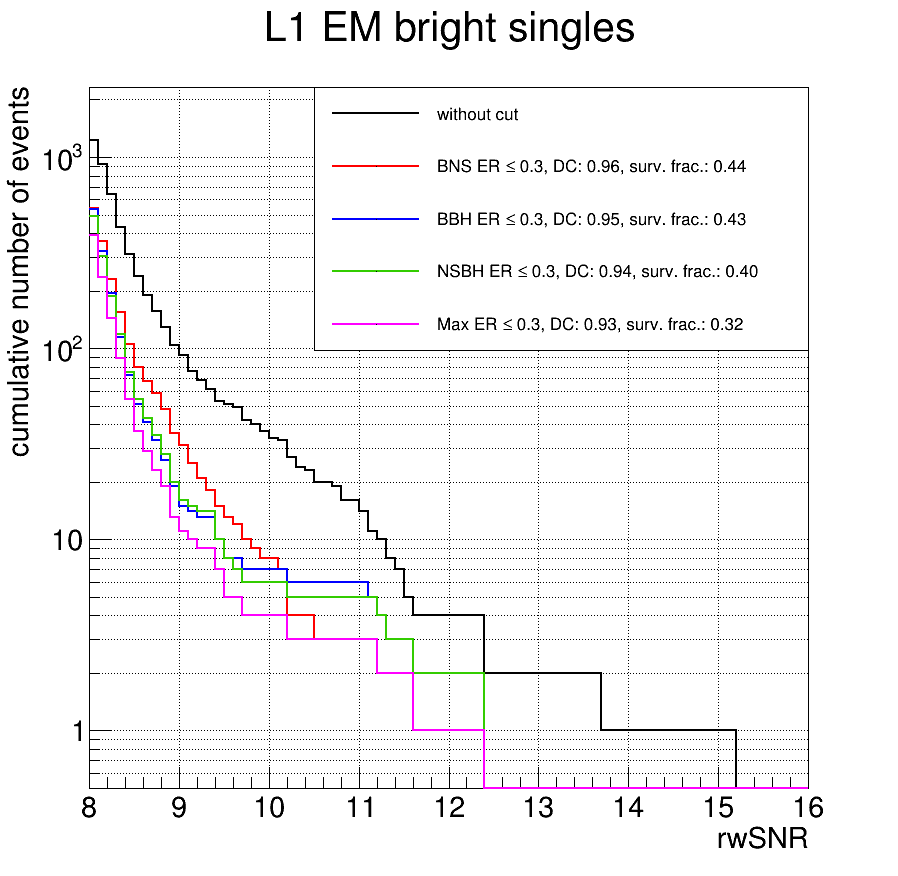
\includegraphics[width=\linewidth]{sectionSelection/plotsEMbright/cCumL1_er.png}
%     \captionof{figure}{Cumulative rwSNR distribution of O3 L1 background EM bright single detector triggers for various cuts on the excess rate. The legend also indicates in each case the remaining duty cycle (DC) and surviving fraction of single detector triggers.}
%     \label{fig:cut_erw_embright_L1}
%   \end{minipage}
%   \hfill
%   \vspace{5mm}
%   % 
%   \begin{minipage}{0.45\linewidth}
%     \centering
%     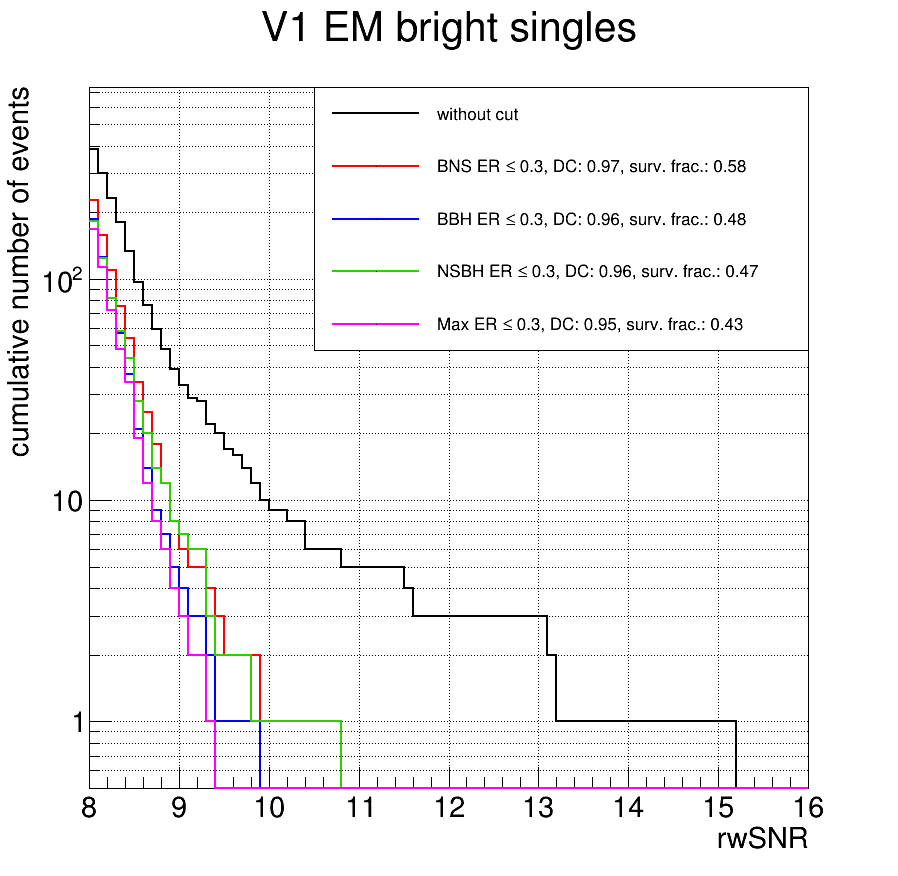
\includegraphics[width=\linewidth]{sectionSelection/plotsEMbright/cCumV1_er.png}
%     \captionof{figure}{Cumulative rwSNR distribution of O3 V1 background EM bright single detector triggers for various cuts on the excess rate. The legend also indicates in each case the remaining duty cycle (DC) and surviving fraction of single detector triggers.}
%     \label{fig:cut_erw_embright_V1}
%   \end{minipage}
%   \hfill
% \end{figure}
%%

\begin{figure}
  \centering
  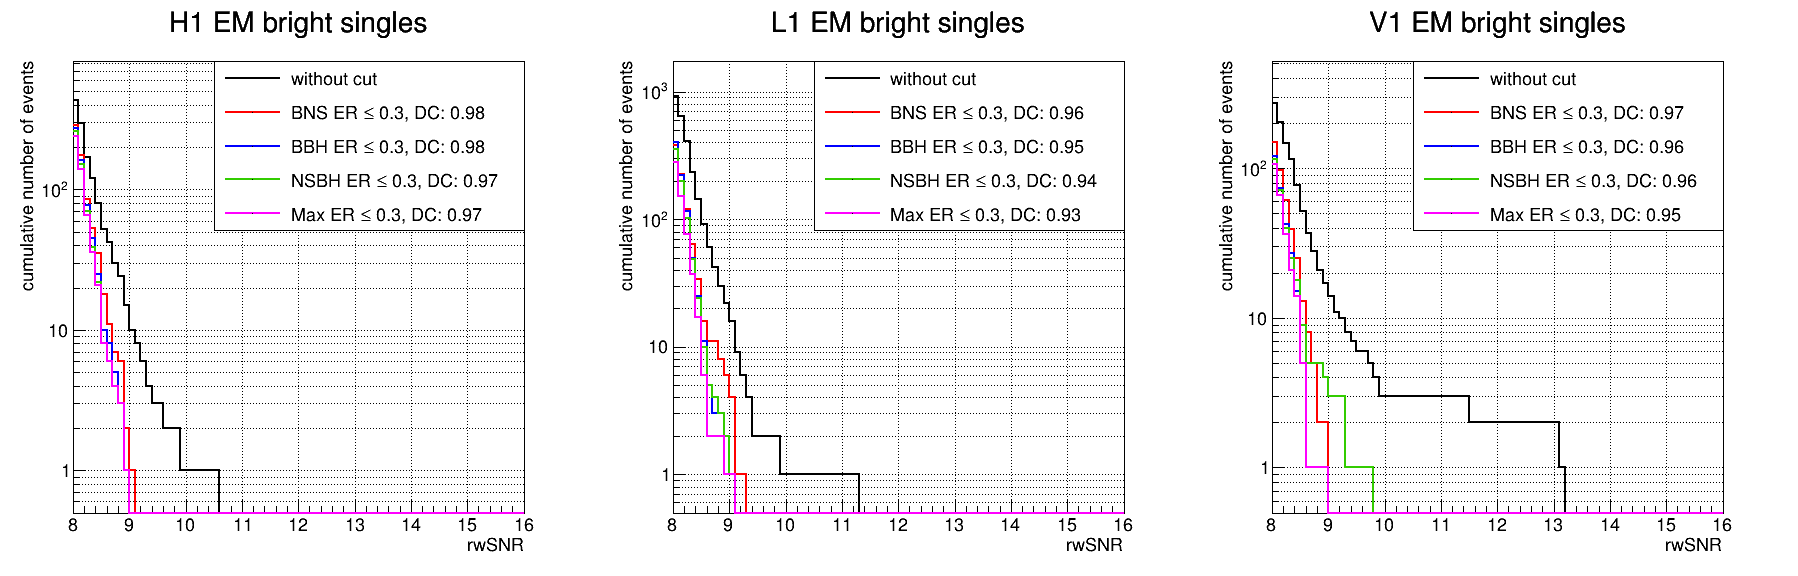
\includegraphics[width=\linewidth]{sectionSelection/plotsEMbright/cCumER.png}
  \caption{Cumulative rwSNR distribution of O3 background EM bright single detector triggers for a cut on the different excess rates. The legend also indicates in each case the remaining duty cycle (DC).}
  \label{fig:cut_erw_embright}
\end{figure}


\begin{figure}
  \centering
  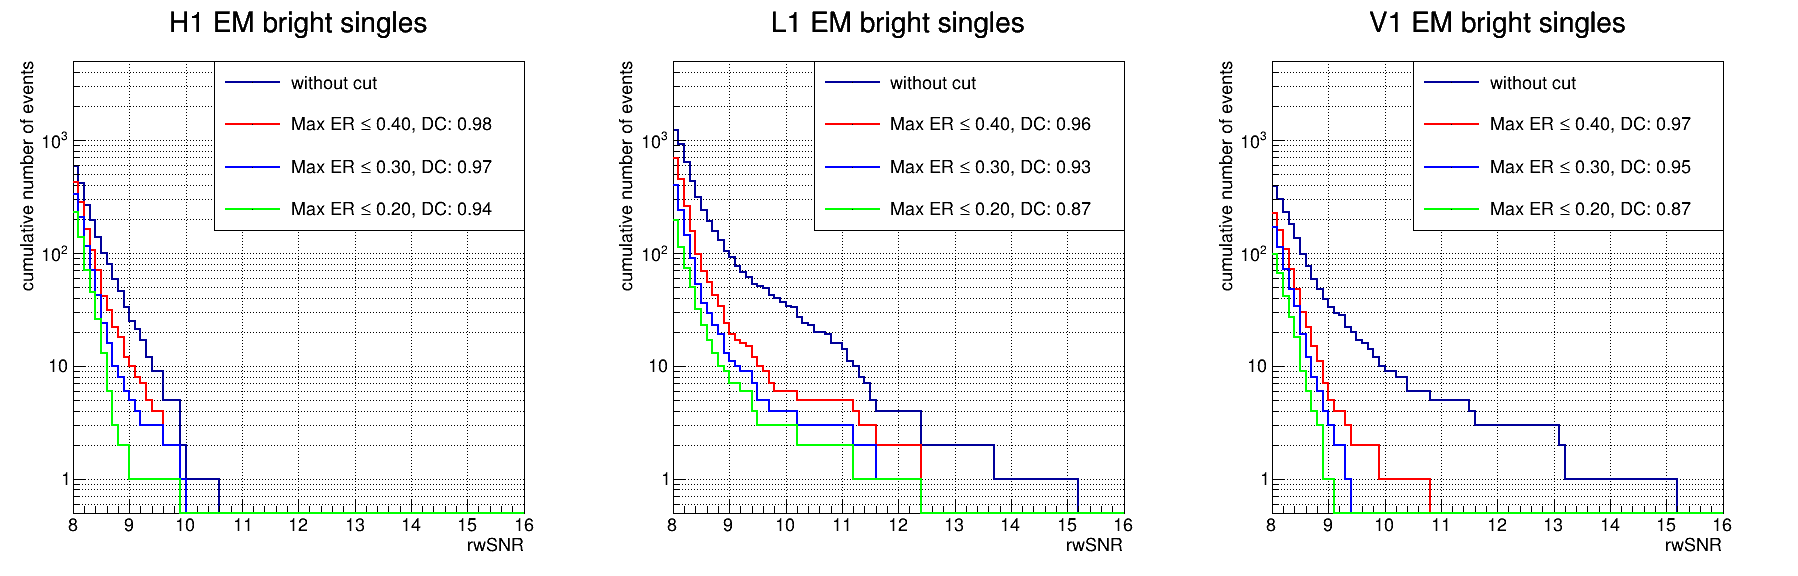
\includegraphics[width=\linewidth]{sectionSelection/plotsEMbright/cCumulERcut.png}
  \caption{Cumulative rwSNR distribution of O3 background EM bright single detector triggers for different excess rate cuts and remaining duty cycle (DC) for each.}
  \label{fig:embright_ercut}
\end{figure}



%% 
\begin{figure}[hb]
  \centering
  \begin{minipage}{0.45\linewidth}
    \centering
    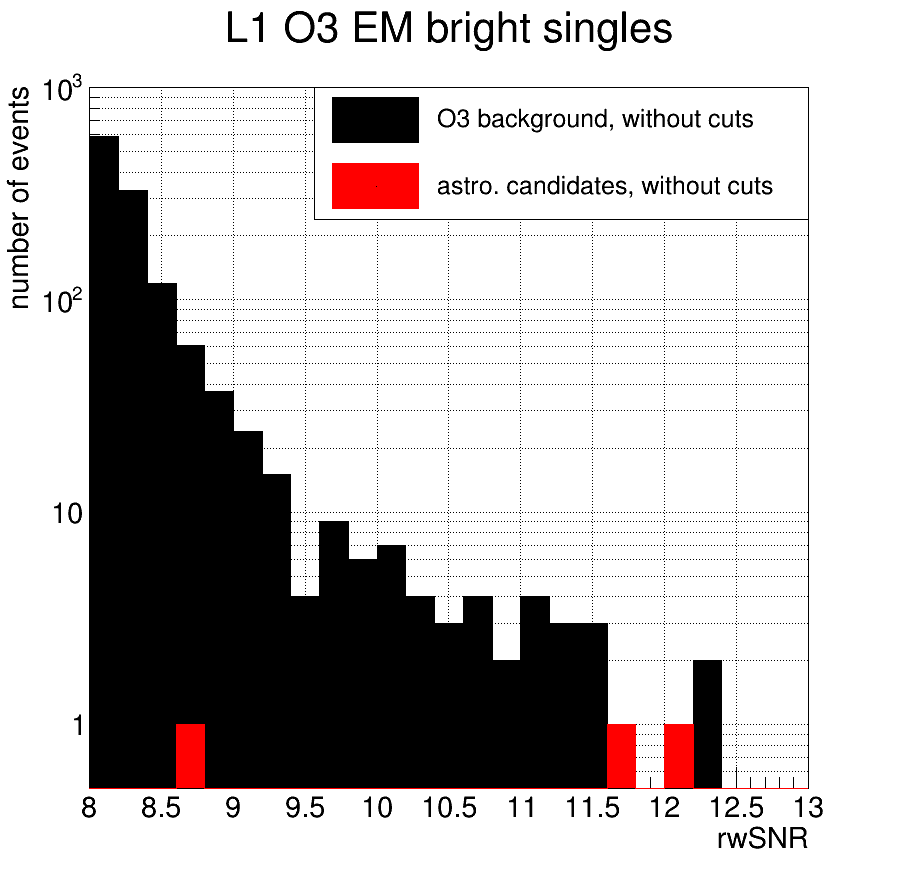
\includegraphics[width=\linewidth]{sectionSelection/plotsEMbright/cL1_O3_beforeCut.png}
    \label{fig:embright_astro_beforecut}
  \end{minipage}
  \hfill
  % 
  \begin{minipage}{0.45\linewidth}
    \centering
    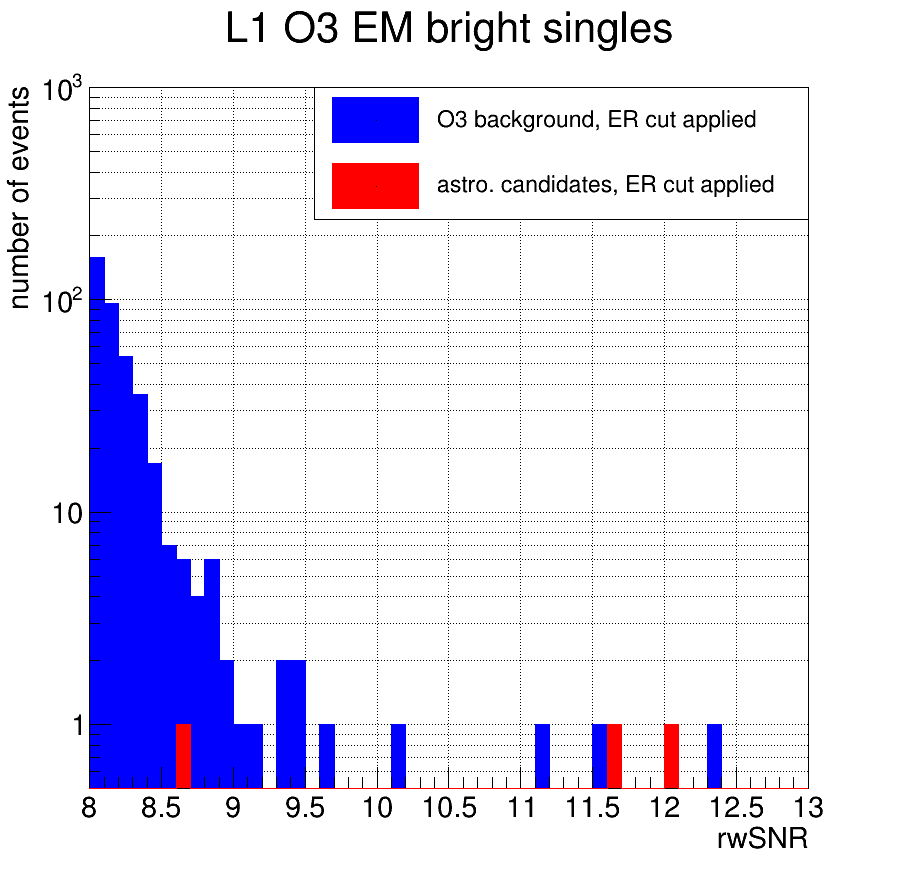
\includegraphics[width=\linewidth]{sectionSelection/plotsEMbright/cL1_O3_afterCutER.png}
    \label{fig:embright_astro_aftercut}
  \end{minipage}
  \hfill
  \caption{rwSNR distribution of O3 background EM bright single detector triggers and astrophysical candidates before (left) and after (right) applying the excess rate cut.}
  \label{fig:embright_astro_ercut}
\end{figure}


\begin{table}
  \centering
  \begin{tabular}{c|c|c|c}
    Name & GPS time & rwSNR & ER \\ \hline
    GW190425 & 1240215503.027 & 12.07 & 0 \\
    GW200105\_162426 & 1262276684.066 & 11.69 & 0 \\
    GW200115\_042309 & 1263097407.744 & 8.63 & 0.066 \\
  \end{tabular}
  \caption{MBTA's EM bright single detector triggers associated to GWTC-2.1 and GWTC-3 astrophysical events.}
  \label{tab:astro}
\end{table}




\clearpage\newpage
\subsubsection{Excess rate on EM dark single detector triggers}
\label{sec:emdark_er}

Since for the EM dark region we have more single detector triggers ($>10^3$ per detector) and we are looking at higher masses, we wonder whether we should be stricter on the excess rate cut.
To this end we will also investigate cuts below ER $=0.3$.
Figure \ref{fig:emdark_ercut} shows the SNR distribution of the EM dark population for different values of cut on the max ER.
We see that cutting on the max ER allows for some background rejection but the value of the cut has little impact unlike for EM bright triggers.
Since being more restrictive does not make things significantly better and aggressive cuts can be dangerous (risk of missing astrophysical events due to lower duty cycle), we settle for a cut on the excess rate at 0.3.
The comparison with the astrophysical candidates is shown in figure \ref{fig:emdark_astro_ercut}.
%% 
\begin{figure}
  \centering
  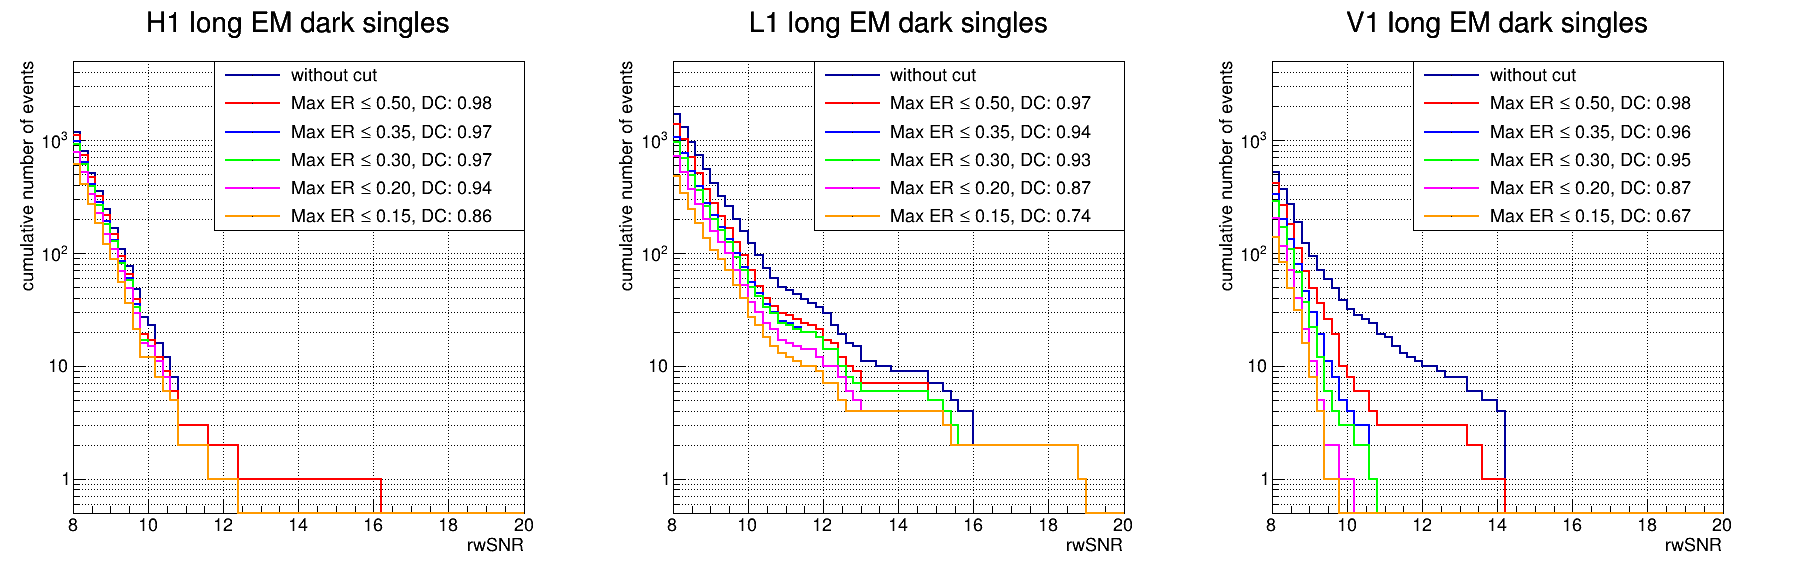
\includegraphics[width=\linewidth]{sectionSelection/plotsEMdark/cCumulERcut.png}
  \caption{Different excess rate cuts on O3 long EM dark single detector triggers and remaining duty cycle (DC) for each.}
  \label{fig:emdark_ercut}
\end{figure}
%% 

%%
\begin{figure}[hb]
  \centering
  \begin{minipage}{0.45\linewidth}
    \centering
    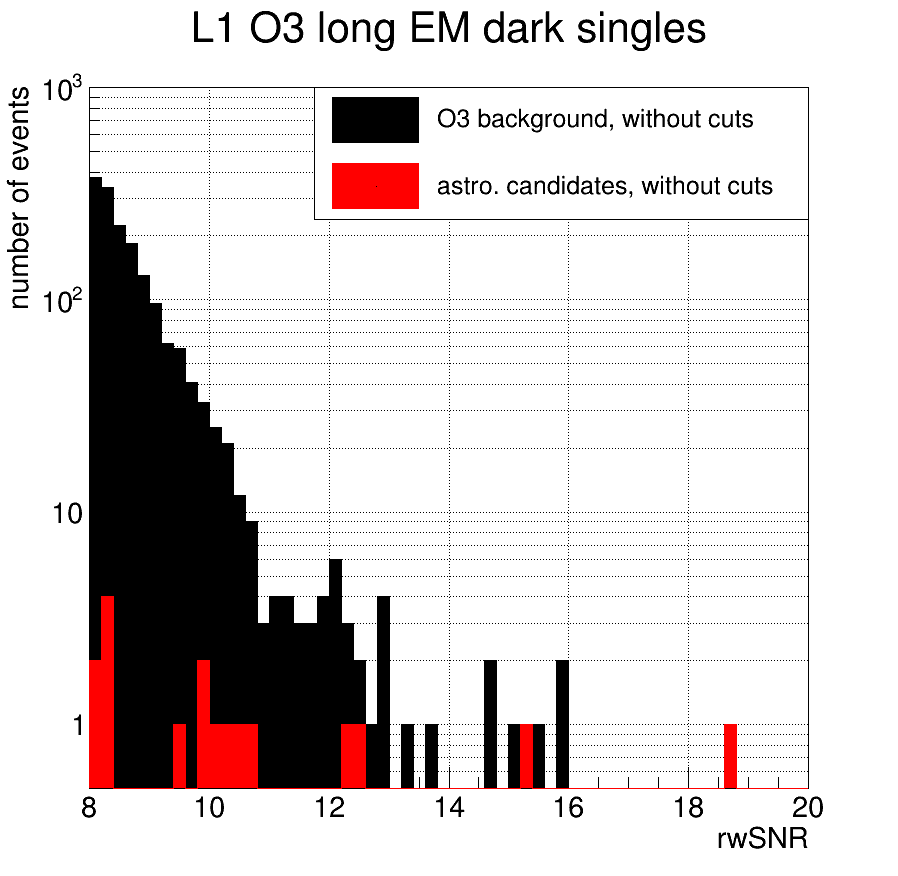
\includegraphics[width=\linewidth]{sectionSelection/plotsEMdark/cL1_O3_beforeCut.png}
    \label{fig:emdark_astro_beforecutER}
  \end{minipage}
  \hfill
  % 
  \begin{minipage}{0.45\linewidth}
    \centering
    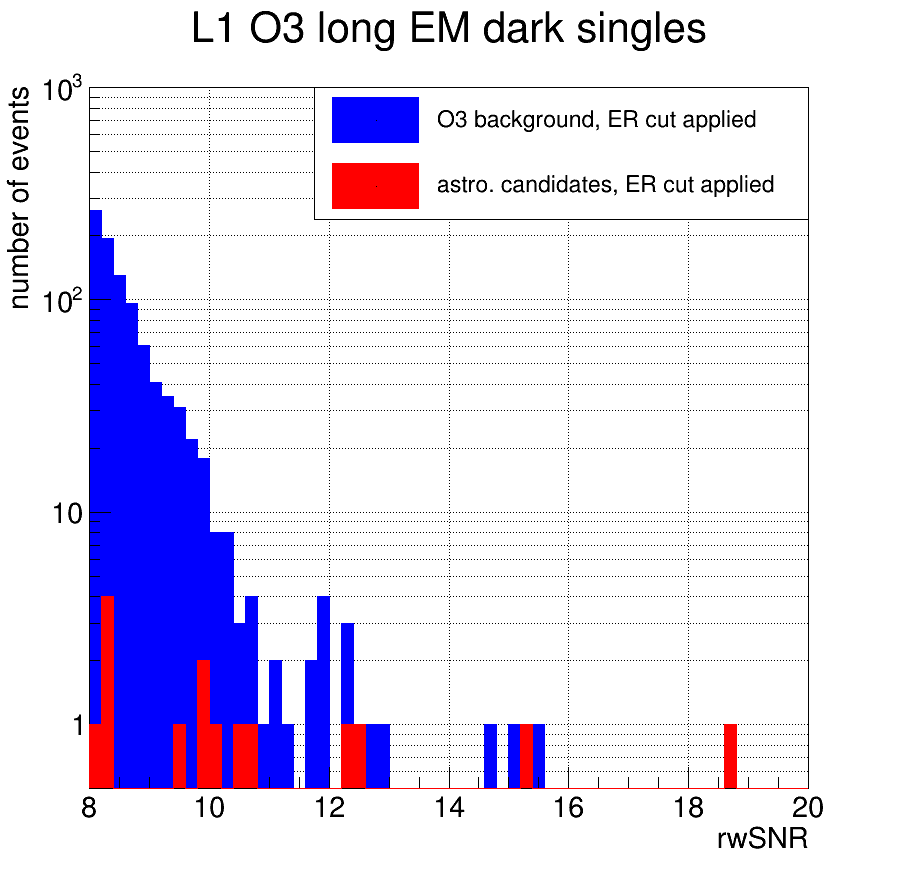
\includegraphics[width=\linewidth]{sectionSelection/plotsEMdark/cL1_O3_afterCutER.png}
    \label{fig:emdark_astro_anyERonly}
  \end{minipage}
  \hfill
  \caption{rwSNR distribution of O3 background EM dark single detector triggers and astrophysical candidates before (left) and after (right) applying the excess rate cut.}
  \label{fig:emdark_astro_ercut}
\end{figure}






%%%%%%%%%% 
\clearpage\newpage
\subsection{Need of a larger cut on the excess rate and gating}
\label{sec:selec_gating}
We wondered at some point whether the time at which we take the excess rate for the single detector triggers was of high importance for our cut, or if a shift of a few seconds would not change much.
The reason for this thought is that the ER is computed as a median value over \SI{10}{s} so a shift in time may bring some differences.
To investigate this question, we apply the selection with different time offset, as presented in figure \ref{fig:erTimeShift}.
We see that the delay does not matter much in H1 and V1 but there are some more significant differences in L1 for both EM bright and long EM dark single detector triggers.
Since this effect appears only in L1 it is not clear at this point wether it is actually due to the delay introduced for the excess rate.
We can further investigate the matter by looking at events with large rwSNR that were not rejected previously by the ER cut. Figure \ref{fig:diagPlots} shows the excess rate vs time with indication of gated times.
We see that there is clearly an issue with those single detector triggers: the presence of gating close to the trigger indicates a bad period of time and the spike in the excess rate right after the trigger explains why shifting the time at which we take the excess rate had an impact on the SNR distribution.
Further investigation showed that these single detector triggers were not isolated cases and many other displayed such behaviour.
%% 
\begin{figure}
  \centering
  \begin{minipage}{\linewidth}
    \centering
    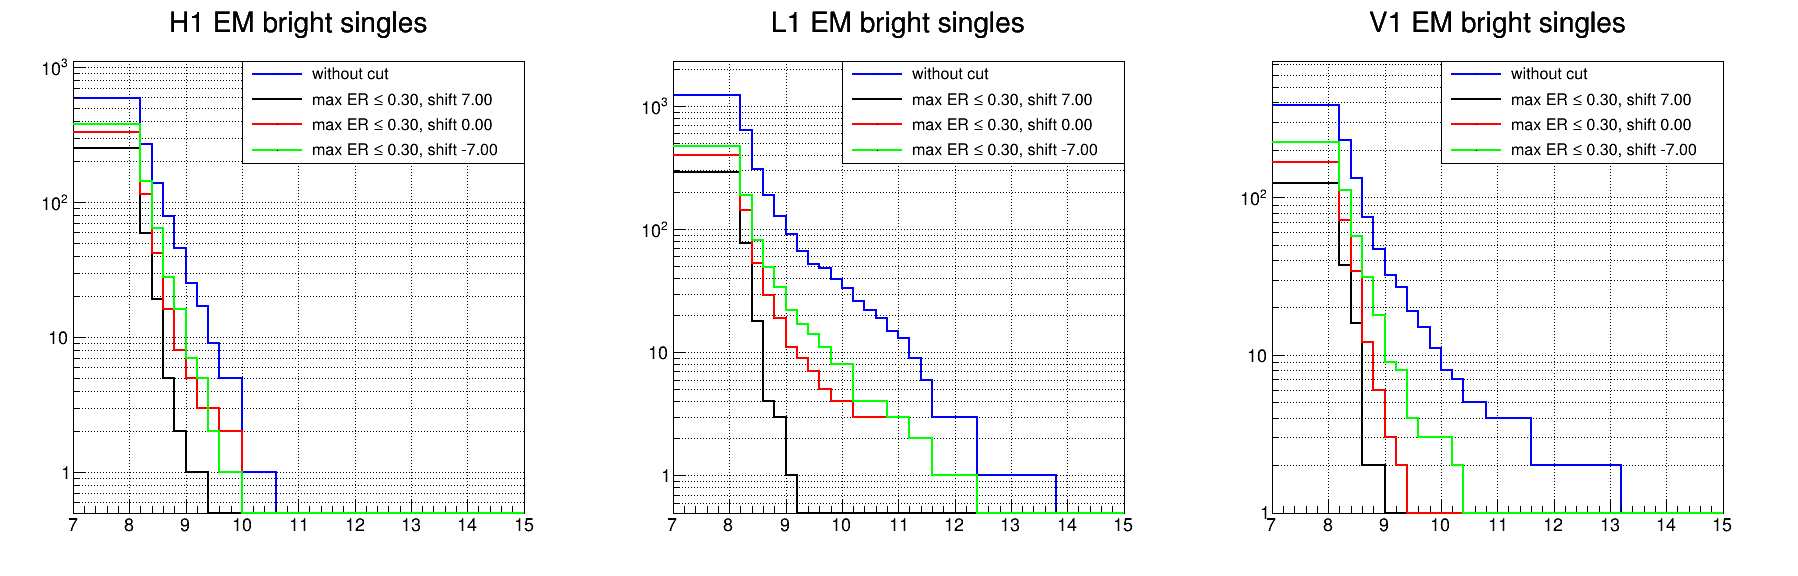
\includegraphics[width=\textwidth]{sectionSelection/plotsAroundSingles/cCumulERtimeShift_bright.png}    
  \end{minipage}
  \hfill
  \begin{minipage}{\linewidth}
    \centering
    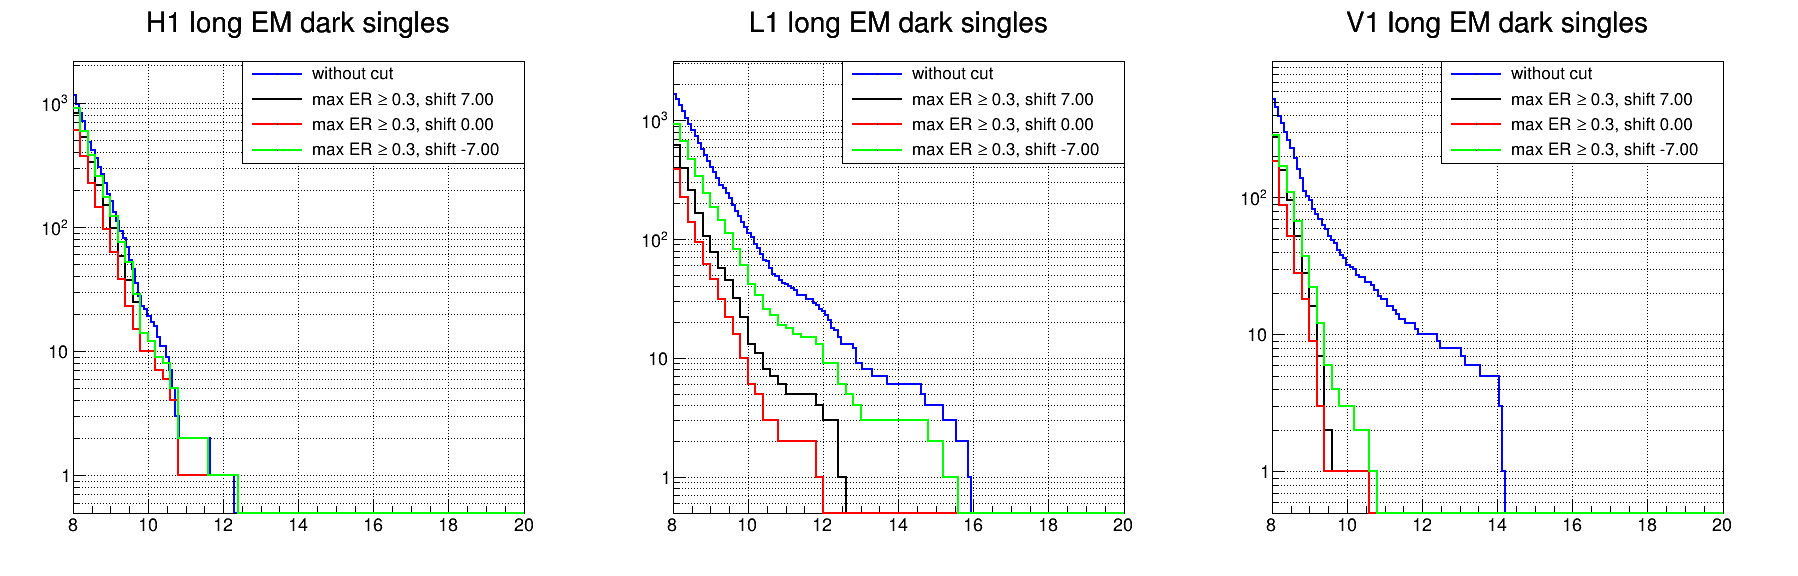
\includegraphics[width=\textwidth]{sectionSelection/plotsAroundSingles/cCumulERtimeShift.png}
  \end{minipage}
  \caption{rwSNR distribution with different time shifts on the excess rate. EM bright (top) and long EM dark (bottom) single detector triggers.}
  \label{fig:erTimeShift}
\end{figure}
% 
% 

\begin{figure}
  \centering
  \begin{minipage}{\linewidth}
    \centering
    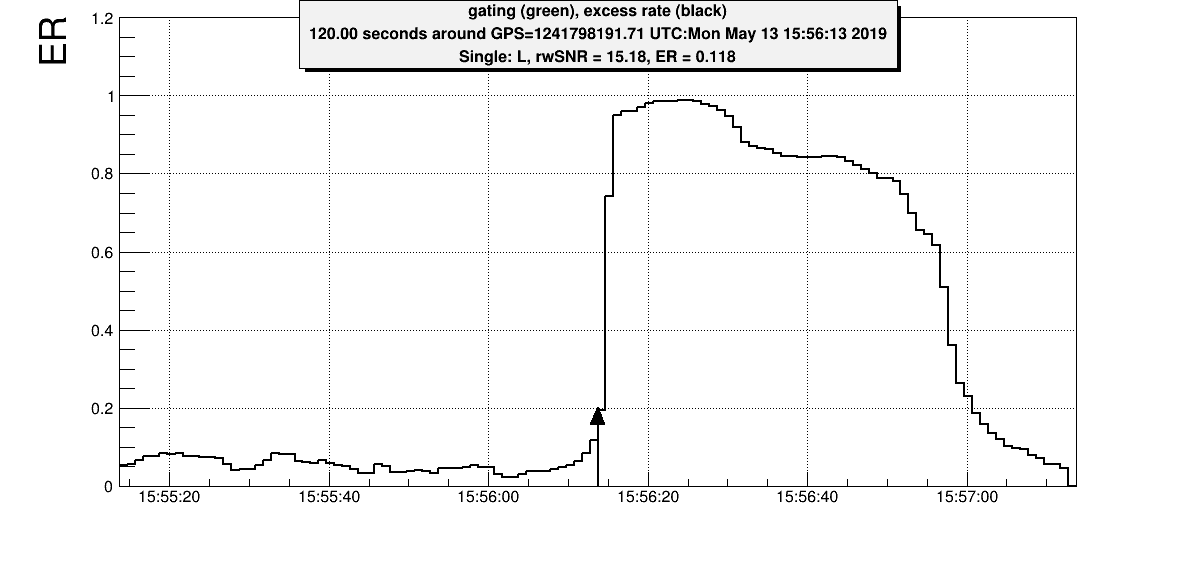
\includegraphics[width=0.8\linewidth]{sectionSelection/plotsAroundSingles/1241798191-71_gatingER.png}
  \end{minipage}
% 
  \begin{minipage}{\linewidth}
    \centering
    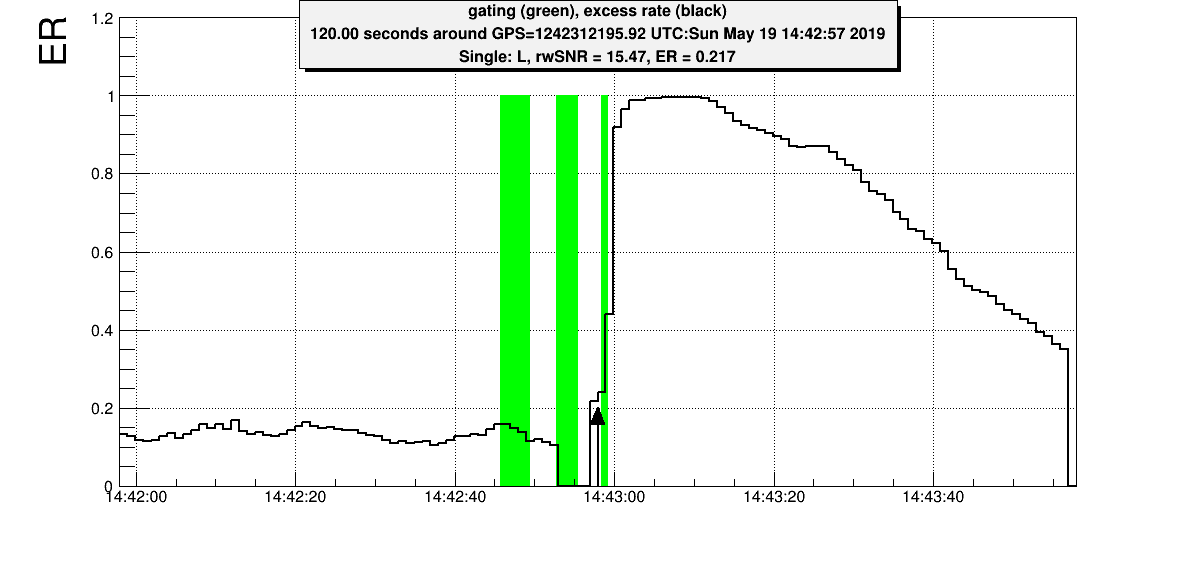
\includegraphics[width=0.8\linewidth]{sectionSelection/plotsAroundSingles/1242312195-92_gatingER.png}
  \end{minipage}
% 
  \begin{minipage}{\linewidth}
    \centering
    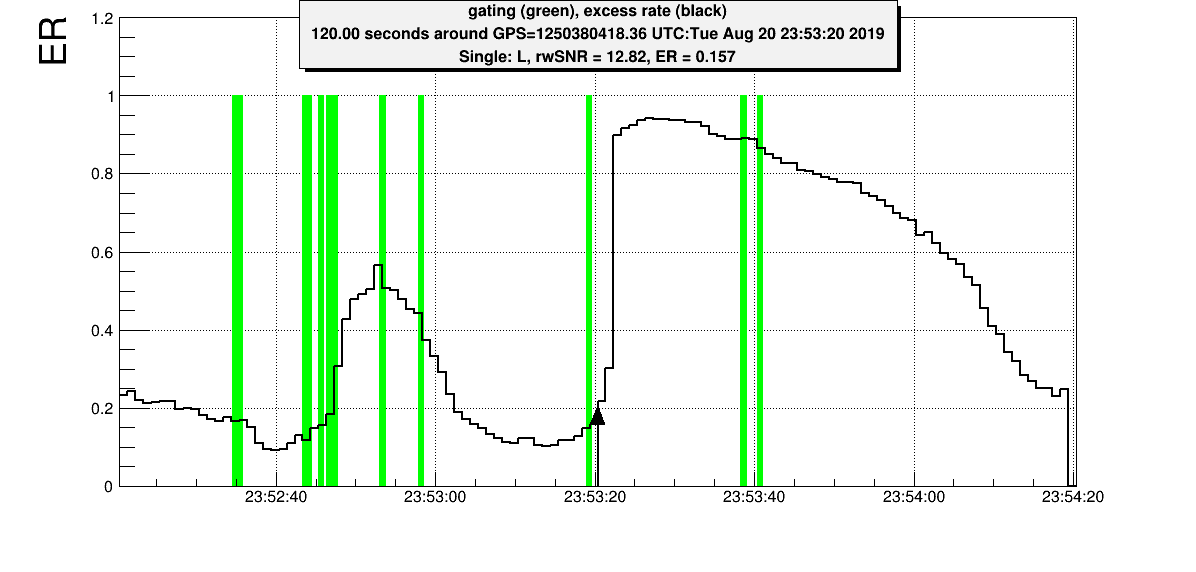
\includegraphics[width=0.8\linewidth]{sectionSelection/plotsAroundSingles/1250380418-35_gatingER.png}
  \end{minipage}
  \caption{Gating and excess rate around some single detector triggers in L1. The time of the trigger is indicated by an arrow each time.}
  \label{fig:diagPlots}
\end{figure}
%% 

We therefore decide to reject any single detector trigger for which a gated time is found within $[-20,+5]$ \si{s} and we require that the excess rate should not exceed 0.3 in the time window $[-7;7]$ \si{s} centered on the trigger. The result is shown in figures \ref{fig:embright_cutGating}, \ref{fig:embright_cutMoreER} for the EM bright single detector triggers (to be compared to figure \ref{fig:embright_astro_aftercutER}) and \ref{fig:emdark_cutGating}, \ref{fig:emdark_cutMoreER} for the EM dark single detector triggers (to be compared with figure \ref{fig:emdark_astro_aftercutER}).
As can be seen the tail of the distribution is cleaner and the total number of events has decreased.
The total loss of duty cycle for O3 due to the application of those cuts is 9.1\% in H1, 15.4\% in L1 and 9.8\% in V1.

As a final plot for the selection we show the comparison of the EM bright and long dark triggers distribution with the Gaussian noise after the selection in figures \ref{fig:compare_bright_gaus_selec} and \ref{fig:compare_longDark_gaus_selec}.
We also show the template duration versus rwSNR distribution of EM dark single detector triggers in figure \ref{fig:emdark_snrTempDur_allcut} to confirm that the separation between long and short templates still holds.
The separation based on the duration is still meaningful after applying the selection as we can still see some noisy templates with very short duration.

%% 
\begin{figure}
  \centering
  \begin{minipage}{0.45\linewidth}
    \centering
    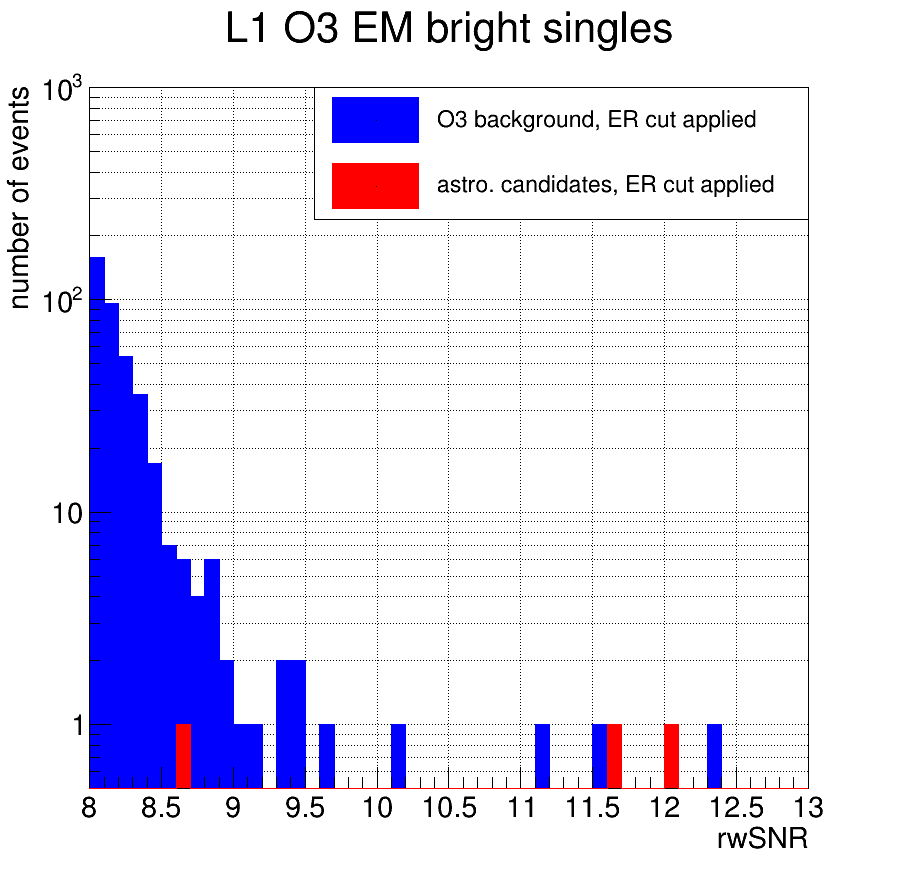
\includegraphics[width=\linewidth]{sectionSelection/plotsEMbright/cL1_O3_afterCutER.png}
    \captionof{figure}{rwSNR distribution for EM bright single detector triggers with the simple excess rate cut described in section \ref{sec:emdark_er}.}
    \label{fig:embright_astro_aftercutER}
  \end{minipage}
  \hfill
  % 
  \begin{minipage}{0.45\linewidth}
    \centering
    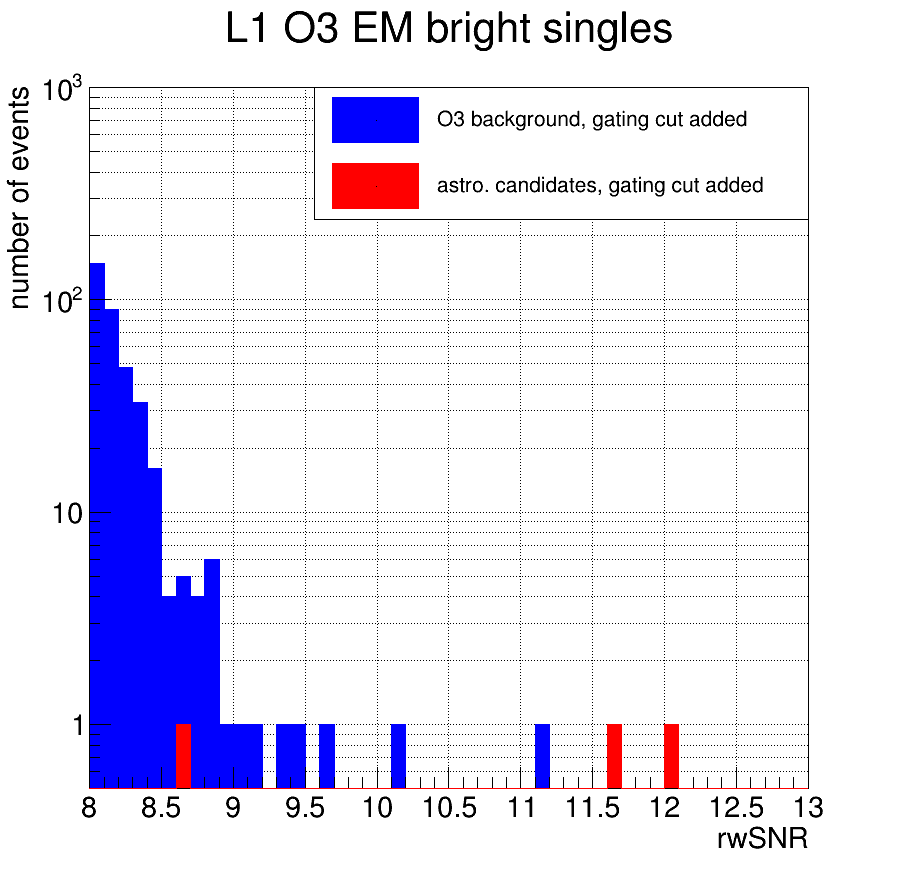
\includegraphics[width=\linewidth]{sectionSelection/plotsEMbright/cL1_O3_afterCutGating.png}
    \captionof{figure}{rwSNR distribution for EM bright single detector triggers after applying the cut on the gating.}
    \label{fig:embright_cutGating}
  \end{minipage}
  \hfill
  % 
  \begin{minipage}{0.45\linewidth}
    \centering
    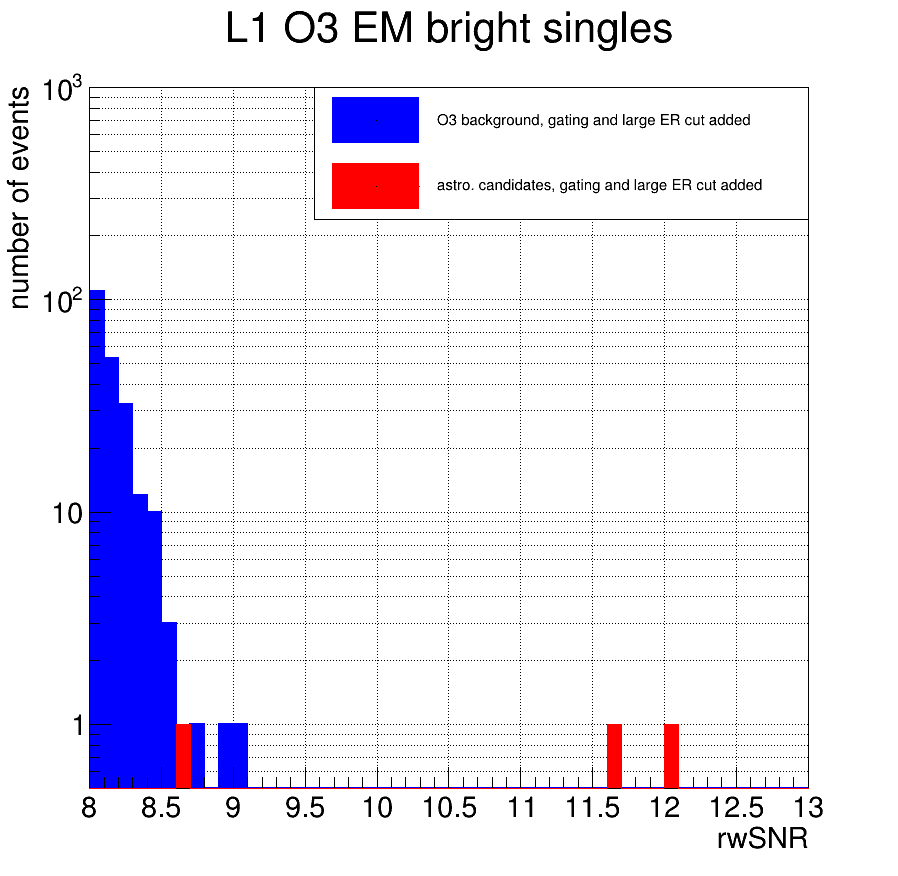
\includegraphics[width=\linewidth]{sectionSelection/plotsEMbright/cL1_O3_afterCutMoreER.png}
    \captionof{figure}{rwSNR distribution for EM bright single detector triggers after applying the larger cut on the excess rate in addition to the cut on the gating.}
    \label{fig:embright_cutMoreER}
  \end{minipage}
  \hfill
\end{figure}
%% 

%% 
\begin{figure}
  \centering
  \begin{minipage}{0.45\linewidth}
    \centering
    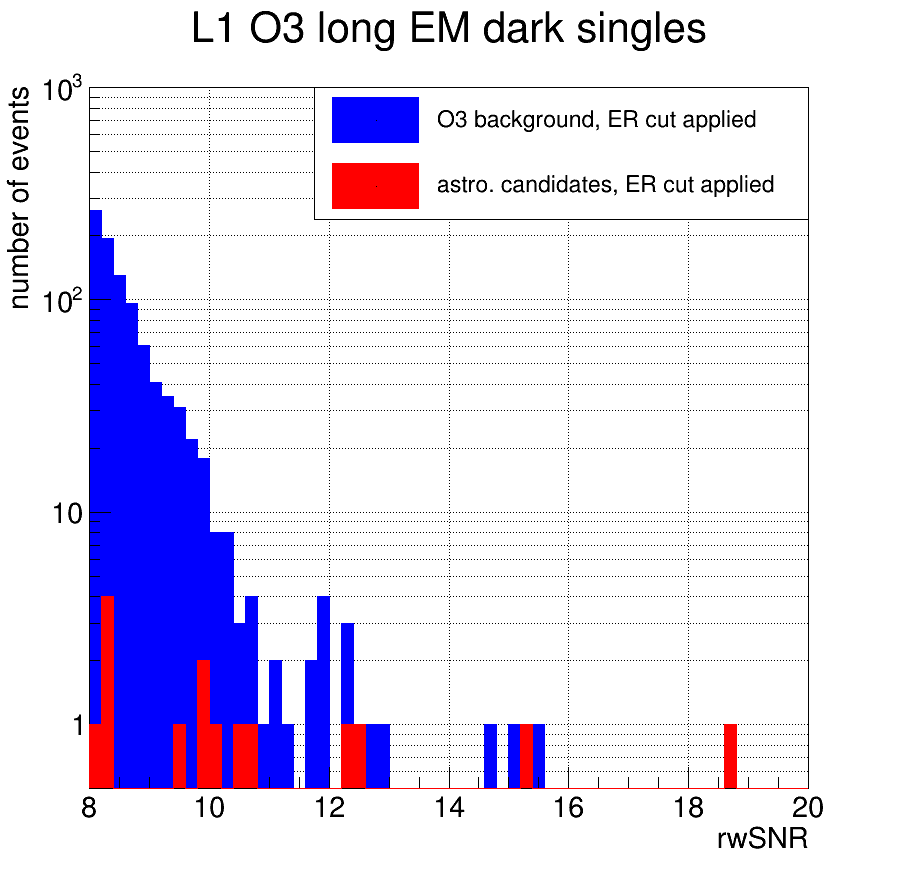
\includegraphics[width=\linewidth]{sectionSelection/plotsEMdark/cL1_O3_afterCutER.png}
    \captionof{figure}{O3 long EM dark single detector triggers: SNR distribution with the simple excess rate cut described in section \ref{sec:emdark_er}.}
    \label{fig:emdark_astro_aftercutER}
  \end{minipage}
  \hfill
  % 
  \begin{minipage}{0.45\linewidth}
    \centering
    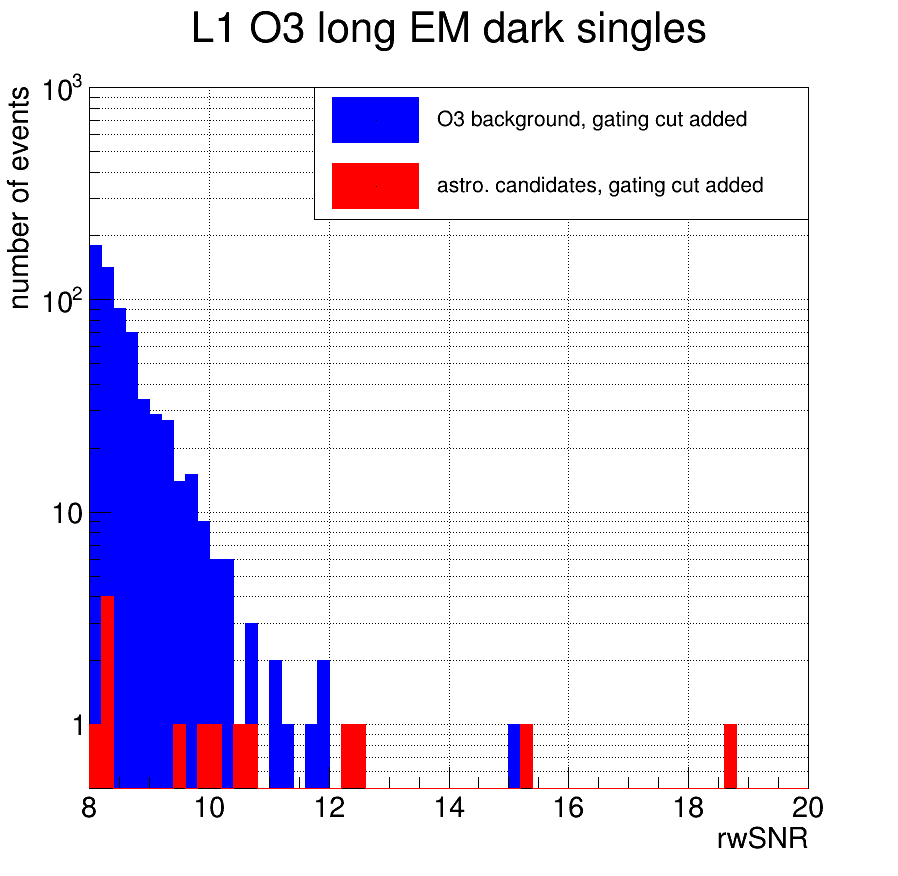
\includegraphics[width=\linewidth]{sectionSelection/plotsEMdark/cL1_O3_afterCutGating.png}
    \captionof{figure}{O3 long EM dark single detector triggers: SNR distribution after applying the cut on the gating.}
    \label{fig:emdark_cutGating}
  \end{minipage}
  \hfill
  % 
  \begin{minipage}{0.45\linewidth}
    \centering
    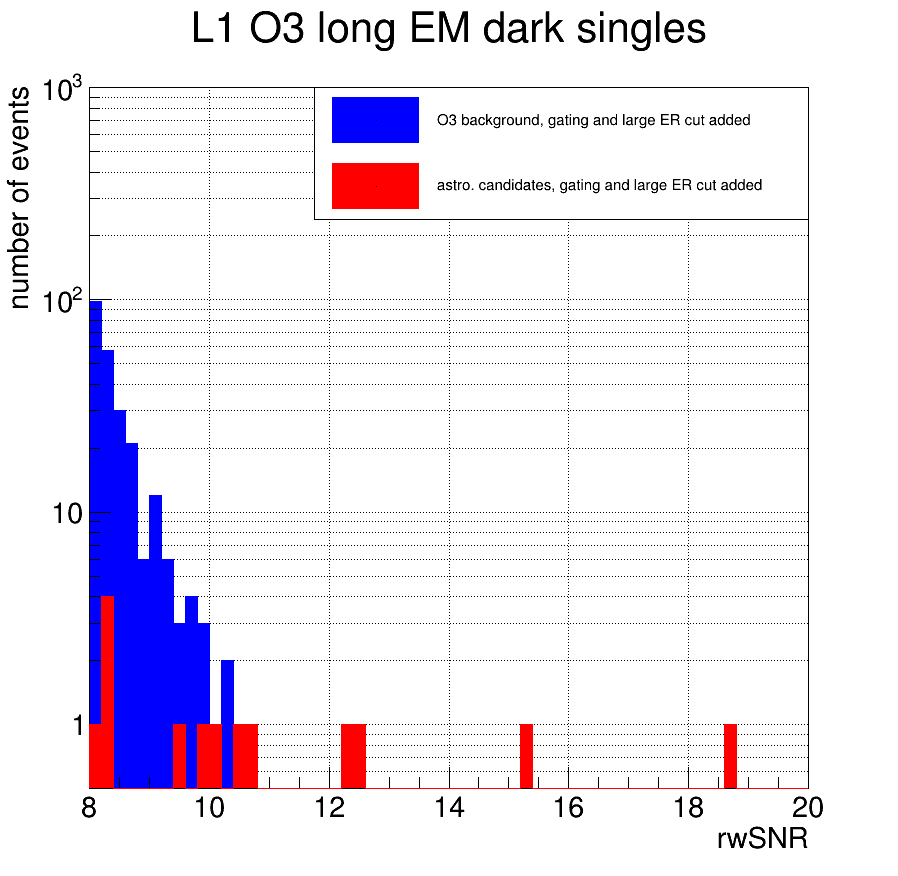
\includegraphics[width=\linewidth]{sectionSelection/plotsEMdark/cL1_O3_afterCutMoreER.png}
    \captionof{figure}{O3 long EM dark single detector triggers: SNR distribution after applying the larger cut on the excess rate in addition to the cut on the gating.}
    \label{fig:emdark_cutMoreER}
  \end{minipage}
  \hfill
\end{figure}
% 
% 
\begin{figure}
  \centering
  \includegraphics[width=\textwidth]{sectionSelection/plotsEMbright/cPosterAllCut.png}
  \caption{rwSNR distribution: O3 EM bright single detector triggers after selection (gating and wide ER cut) vs Gaussian noise}
  \label{fig:compare_bright_gaus_selec}
\end{figure}
% 
%
\begin{figure}
  \centering
  \includegraphics[width=\textwidth]{sectionSelection/plotsEMdark/cPosterAllCut.png}
  \caption{rwSNR distribution: O3 Long EM dark single detector triggers after selection (gating and wide ER cut) vs Gaussian noise}
  \label{fig:compare_longDark_gaus_selec}
\end{figure}
% 
%


%% 
\begin{figure}
  \centering
  \includegraphics[width=\linewidth]{sectionSelection/plotsEMdark/cSnrTempDurAllCut.png}
  \caption{Distribution of the EM dark single detector triggers in the template duration vs rwSNR plane. The cuts on the gating and excess rate are applied. A few short templates are still triggered very often, showing as vertical lines.}
  \label{fig:emdark_snrTempDur_allcut}
\end{figure}
%% 



\clearpage\newpage
\subsection{Search sensitivity improvement}
\label{sec:reweightER}

We have seen that we can reject background by cutting on the excess rate and gating at the cost of some duty cycle.
We want to know how much was gained in terms of efficiency of the search.

One way to answer is by looking at the Volume-Time (VT) (see section \ref{sec:detector}).
This VT is roughly proportional to the number of detections.
The volume scales with the distance cubed, which in turn scales with the inverse of the SNR threshold (eq. \ref{eq:horizon}) (or rwSNR in the present case).
Having lower background means that astrophysical signals with smaller rwSNRs can pass the threshold for detection.
This means an increase in volume.
Hence, we have on one side a loss in observing time and on the other a gain in volume.
We therefore need to estimate both to anwser the initial question.

As mentioned previously, the effective observing time loss caused by the application of the selection is 9.1\% in H1, 15.4\% in L1 and 9.8\% in V1.
Note that during these times with excess rate, the search is less efficient because of the reweighting and there is already some VT loss.
Therefore when cutting these times, the VT reduction is less than the sole observing time loss.

Looking at EM bright single detector triggers in L1 (figure \ref{fig:embright_rankstat_allcut}) and considering a FAR thresold of 2 per year, the ranking statitstics threshold using the simple reweighting would be $\sim 11.2$.
When applying the selection criteria this threshold becomes $\sim 8.8$.
Thus, in first approximation, the gain in volume is $(11.2/8.8)^3-1 = 106.2\%$.
Following the same reasoning, the improvement in H1 and V1 is $(9.5/8.6)^3-1 = 34.8\%$ and $(9.4/8.5)^3-1 = 35.2\%$ respectively.
This gain is much larger than the loss in duty cycle, validating the use of the selection criteria.
The same conclusion can be derived from figure \ref{fig:emdark_rankstat_allcut} for long EM dark single detector triggers.

% Figure \ref{fig:embright_rankstat_allcut} shows the ranking statistics distribution of the EM bright singles detector triggers for a simple reweighting using the ER and for the application of the selection criteria defined in this section.

\begin{figure}[ht]
  \centering
  \includegraphics[width=\linewidth]{sectionSelection/plotsEMbright/cRankStatCutAll.png}
  \caption{Reweighting vs cutting  on the excess rate for O3 EM bright single detector triggers : gating and wide ER cuts.}
  \label{fig:embright_rankstat_allcut}
\end{figure}
% 
\begin{figure}[ht]
  \centering
  \includegraphics[width=\linewidth]{sectionSelection/plotsEMdark/cRankStatCutAll.png}
  \caption{Reweighting vs cutting on the excess rate for O3 long EM dark single detector triggers : gating and wide ER cuts.}
  \label{fig:emdark_rankstat_allcut}
\end{figure}




%%%%%%%%%% 
\clearpage\newpage
\subsubsection{Computation of a new ER in anticipation for O4 bank}
\label{sec:newER}
We have shown what can be achieved by applying cuts on the excess rate and the gating.
We have until now used the maximum of the 3 search regions excess rates as explained in section \ref{sec:correl_ER}, but for O4 we will have only one region.
In this section we explore how the result will change with an excess rate computed on only one region.

%Since the excess rates are correlated, is it really useful to distinguish between the search regions to compute it?
%Can we compute a single global value for the excess rate in a detector, as would be the case during O4?\textcolor{red}{Est ce que cette question n'arrive pas trop tard}
%The answer is yes, and the way to compute it is pretty straightforward.
The excess rate is computed from the trigger rates before and after data quality checks following equation (\ref{eq:ER}).
For O3 it is computed for each search region by taking independently the rates for each of them.
To achieve our goal we can simply add up those rates  to have one total rate before and after quality checks.
We can then compute a single excess rate following equation \ref{eq:ER}.
Figure \ref{fig:compareOldNewER} shows the comparison between the maximum of the three search regions' excess rates and the newly computed excess rate.
As can be seen the new one has a tendency to be lower than the maximum ER.
This is expected since in the case where one of the 3 ER is high while the other two have smaller values, the maximum will be high while our new ER will be closer to a mean value of the 3.

We can now apply the same cuts as before with a substitution of the max ER by the new ER to compare the effect of both.
The result is shown in figures \ref{fig:newER_embright} and \ref{fig:newER_emdarkLong} for EM bright and long EM dark single detector triggers respectively.
As can be see, there is little difference between the 2 excess rate.
A few more events survive the cuts when using the new ER since it is generally lower but it does not significantly affects the tail of the distributions.
We can also note that using the new ER, we retrieve one more astrophysical event among the short EM dark single detector triggers in L1.
Figures \ref{fig:newER_gaus_bright} and \ref{fig:newER_gaus_darkLong} show the comparison with Gaussian noise after the full selection.
The total loss of duty cycle when applying the cut on the gating and new ER is of 6\%, 14.1\% and 9\% for H1, L1 and V1 respectively.
For comparison, using the old (max) ER, the loss was of 9.1\%, 15.4\% and 9.8\% for H1, L1 and V1.
% 
\begin{figure}
  \centering
  \includegraphics[width=\linewidth]{sectionSelection/plotsNewER/cOldNew.png}
  \caption{Comparison between the old max ER and the new ER.}
  \label{fig:compareOldNewER}
\end{figure}
% 
% EM BRIGHT
\begin{figure}
  \centering
  \begin{minipage}{0.45\linewidth}
    \centering
    \includegraphics[width=\linewidth]{sectionSelection/plotsNewER/cL1bright_afterCutER_newER.png}
  \end{minipage}
  \hfill
  % 
  \begin{minipage}{0.45\linewidth}
    \centering
    \includegraphics[width=\linewidth]{sectionSelection/plotsNewER/cL1bright_afterCutMoreER_newER.png}
  \end{minipage}
  \hfill
  \captionof{figure}{rwSNR distributions for L1 O3 EM bright single detector triggers with ER selection (left) and ER+gating selection (right) using the old (max) and new ER (common region).}
  \label{fig:newER_embright}
\end{figure}
% 
% EM DARK LONG
\begin{figure}
  \centering
  \begin{minipage}{0.45\linewidth}
    \centering
    \includegraphics[width=\linewidth]{sectionSelection/plotsNewER/cL1dark_afterCutER_newER.png}
  \end{minipage}
  \hfill
  % 
  \begin{minipage}{0.45\linewidth}
    \centering
    \includegraphics[width=\linewidth]{sectionSelection/plotsNewER/cL1dark_afterCutMoreER_newER.png}
  \end{minipage}
  \hfill
  \captionof{figure}{rwSNR distributions for L1 O3 long EM dark single detector triggers with ER selection (left) and ER+gating selection (right) using the old (max) and new ER (common region).}
  \label{fig:newER_emdarkLong}
\end{figure}
%

% % EM DARK SHORT
% \begin{figure}
%   \centering
%   \begin{minipage}{0.45\linewidth}
%     \centering
%     \includegraphics[width=\linewidth]{sectionSelection/plotsNewER/emDarkShortL1_cutER.png}
%     \captionof{figure}{{\large \textcolor{red}{Retirer les plots dark short?}}Cut on the excess rate on L1 O3 short EM dark single detector triggers using the old (max) and new ER.}
%     \label{fig:newER_emdarkShort_ER}
%   \end{minipage}
%   \hfill
%   % 
%   \begin{minipage}{0.45\linewidth}
%     \centering
%     \includegraphics[width=\linewidth]{sectionSelection/plotsNewER/emDarkShortL1_allCuts.png}
%     \captionof{figure}{Gating and wide excess rate cut on L1 O3 short EM dark single detector triggers using the old (max) and new ER.}
%     \label{fig:newER_emdarkShort_all}
%   \end{minipage}
%   \hfill
% \end{figure}
% % 

% comparison with Gaussian noise
\begin{figure}
  \centering
  \includegraphics[width=\linewidth]{sectionSelection/plotsNewER/cPosterBright_allCut_newER.png}
  \caption{rwSNR distribution: O3 EM bright single detector triggers after selection (gating and wide new ER cuts) vs Gaussian noise}
  \label{fig:newER_gaus_bright}
\end{figure}
% 
\begin{figure}
  \centering
  \includegraphics[width=\linewidth]{sectionSelection/plotsNewER/cPosterDarkLong_allCut_newER.png}
  \caption{rwSNR distribution: O3 Long EM dark single detector triggers after selection (gating and wide new ER cuts) vs Gaussian noise.}
  \label{fig:newER_gaus_darkLong}
\end{figure}
% 
% \begin{figure}
%   \centering
%   \includegraphics[width=\linewidth]{sectionSelection/plotsNewER/cPosterDarkShort_allCut_newER.png}
%   \caption{Short EM bright single detector triggers: O3 after selection (gating \& wide new ER cuts) vs Gaussian noise (scaled to the total observation time of O3)}
%   \label{fig:newER_gaus_darkShort}
% \end{figure}
% 





% \clearpage
% \newpage
% {\large \textcolor{red}{LEFTOVERS PLOTS}}
% {\large \textcolor{red}{A priori plus nécéssaires?}}
% %% 
% \begin{figure}
%   \centering
%   \begin{minipage}{0.45\linewidth}
%     \centering
%     \includegraphics[width=\linewidth]{SingleSelection/EMdark/cAnyMoreERL1.png}
%     \captionof{figure}{rwSNR distribution of O3 background EM dark single detector triggers and astrophysical candidates before applying the template duration cut.}
%     \label{fig:emdark_astro_anyTemp}
%   \end{minipage}
%   \hfill
%   % 
%   \begin{minipage}{0.45\linewidth}
%     \centering
%     \includegraphics[width=\linewidth]{SingleSelection/EMdark/cL1_O3_longTemp_afterCutMoreER.png}
%     \captionof{figure}{rwSNR distribution of O3 background EM dark single detector triggers and astrophysical candidates with template duration $\geq$ \SI{0.8}{s}.}
%     \label{fig:emdark_astro_longTemp}
%   \end{minipage}
%   \hfill
%   % 
%   \begin{minipage}{0.45\linewidth}
%     \centering
%     \includegraphics[width=\linewidth]{SingleSelection/EMdark/cL1_O3_shortTemp_afterCutMoreER.png}
%     \captionof{figure}{rwSNR distribution of O3 background EM dark single detector triggers and astrophysical candidates with template duration $<$ \SI{0.8}{s}.}
%     \label{fig:emdark_astro_shortTemp}
%   \end{minipage}
%   \hfill
% \end{figure}
% % 



% %%%%%%%%%% 
% \clearpage\newpage
% \subsection{\textcolor{red}{Test with O4 template bank}}
